%%%%%%%%%%%%%%%%%%%%%%%%%%%%%%%%%%%%%%%%%%%%%%%%%%%%%%%%%%%%%%%%%%%%%%%%%%%%%%%%%%%%%%%%%%%%%%%%%%%%%%%%%%%%%%%%%%%%%%%%%%%%%%%%%%%%%%%%%%%%%
\section{Introduction}\label{sec:ch6_intro}
%%%%%%%%%%%%%%%%%%%%%%%%%%%%%%%%%%%%%%%%%%%%%%%%%%%%%%%%%%%%%%%%%%%%%%%%%%%%%%%%%%%%%%%%%%%%%%%%%%%%%%%%%%%%%%%%%%%%%%%%%%%%%%%%%%%%%%%%%%%%%
In the previous chapter we have discussed the application of kicked optical potentials to vortex lattice carrying condensates. The vortex lattice proved to be very resilient, with the individual vortex positions largely unaffected by the perturbation, apart from some minor oscillations about their equilibrium positions. The global structure of the lattice was preserved, and remained well ordered. It begs the question of how to create a disordered arrangement from this well ordered structure. Given the similarity of vortex lattices to some crystal structures in condensed matter, it is interesting to examine lattice ordering, and investigate the behaviour of the vortex lattice subjected to a defect or vacancy. True crystalline solid-state materials have feature sizes on the order of {\AA}ngstroms, and can be difficult to observe experimentally, especially the appearance of lattice defects. Even more difficult can be the creation of well defined defects within the crystal structures. Cold atomic systems allow for the same fundamental effects to be investigated on mesoscopic scales, and in currently experimentally realisable systems. Here, we will demonstrate the creation of crystal defects in a BEC vortex lattice. With this, an interesting question to ask is if the lattice were to lose a vortex at a specified location, how would the overall system respond?

In Section~\ref{sec:phase} we discussed the use of phase imprinting techniques to modify the condensate phase. While it was discussed that a vortex can be created with the required $\pm 2\pi$ phase winding, phase imprinting can also be used to annihilate a pre-existing vortex. Assuming a vortex with clockwise phase winding, the direct application of a phase profile with counter-clockwise winding can remove the topological charge of the vortex and annihilate it. In this chapter we will examine the use of this technique, and investigate the resulting effects on the vortex lattice order.

This work has been accepted for publication in Physical Review A, with the content referenced therefrom.

%%%%%%%%%%%%%%%%%%%%%%%%%%%%%%%%%%%%%%%%%%%%%%%%%%%%%%%%%%%%%%%%%%%%%%%%%%%%%%%%%%%%%%%%%%%%%%%%%%%%%%%%%%%%%%%%%%%%%%%%%%%%%%%%%%%%%%%%%%%%%
\section{Model}\label{sec:model}
%%%%%%%%%%%%%%%%%%%%%%%%%%%%%%%%%%%%%%%%%%%%%%%%%%%%%%%%%%%%%%%%%%%%%%%%%%%%%%%%%%%%%%%%%%%%%%%%%%%%%%%%%%%%%%%%%%%%%%%%%%%%%%%%%%%%%%%%%%%%%

To investigate the evolution of a vortex lattice subjected to the phase imprinting technique we once again numerically solve the Gross--Pitaevskii equation in two dimensions, assuming a strong confinement along the third axis, following the model given in Sec.~\ref{sec:modelsystem}. This allows us to restrict the dynamics to the $x$--$y$ plane and focus fully on the Abrikosov lattice geometry. In the frame co-rotating with the condensate the nonlinear mean-field equation governing the BEC wave-function is once again given by
\begin{align}
    \textrm{i}\hbar\partial_t \Psi(\mathbf{r},t) = \left[-\frac{\hbar^2}{2m}\nabla^2 + V\left(\mathbf{r}\right)
	+ g_{\textrm{2D}}\vert \Psi(\mathbf{r},t) \vert^2- \Omega L_z \right]\Psi(\mathbf{r},t).
    %\textrm{i}\hbar\partial_t \Psi(\mathbf{r},t) = \bigg[&-\frac{\hbar^2}{2m}\nabla^2 + V\left(\mathbf{r}\right) \nonumber\\
	%&+ g_{2D}\vert \Psi(\mathbf{r},t) \vert^2- \Omega L_z \bigg]\Psi(\mathbf{r},t).
\end{align}

While the Abrikosov ground state is perfectly ordered, removing or adding vortices will lead to disorder in the lattice. Recently, quantifying the disorder of vortex lattices has become an active topic of interest \cite{VTX:Mithun_pra_2016,VTX:Rankonjac_pra_2016}. %These topics are particularly useful as they can allow the study of quantum turbulence in highly controllable systems \cite{Vtx:Neely_prl_2013,Vtx:Kwon_pra_2014,Vtx:Groszek_pra_2016}.
Here, we suggest to quantify the order of the vortex lattice by first determining the position of each vortex by summing the wavefunction phase over adjacent grid sites and locating $\pm 2\pi$ windings. This gives a vortex position estimated to the nearest numerical grid point. A linear least-squares fit is then performed to more accurately determine the vortex core location to sub-grid resolution, as described by Sec.~\ref{sec:vortrack}. This allows us to determine the wavefunction zeroes within the region, and obtain a continuous rather than discrete range of values for the vortex positions. Since tracking many-body dynamics is a difficult problem, we make use of the Delaunay triangulation and Voronoi tessellation techniques from computational geometry to examine the ordering of the the vortex lattice, as introduced in Sec.~\ref{sec:delaunay}. In the ideal triangular Abrikosov lattice, every vortex has 6 nearest neighbours, $l=(0,\ldots,5)$, located at $\theta_l=l\pi/3$ around the polar angle. Any perturbation that breaks this symmetric arrangement can be easily observed using Delaunay triangulation. This technique generates a mesh from the vortex positions, which makes it easy to check for the presence of non 6-fold neighbouring vortices. These vortices are termed as $n$-fold topological lattice defects, where $n$ is the number of connected edges, and dislocation defects can form when, for example, a 5-fold and a 7-fold defect pairs. Since all these structures are easily countable, this method allows us to characterize the effect that a well-defined perturbation has on the lattice. Alternatively, Voronoi tessellations, which can be generated from the Delaunay triangulation and vice versa, make it easy to observe structural changes in the lattice, and are useful for visualising quantities local to the regions of interest.

As unperturbed Abrikosov lattices in BECs are well ordered everywhere in the bulk region \cite{Vtx:Anglin_arxiv_2002} we define the previously mentioned radial boundary at approximately $2/3$ of the maximum density, which corresponds to $r=2\times 10^{-4}$ m from the BEC centre and restrict our analysis to vortices inside it. This leaves an edge boundary of approximately $4a_v$ wide where vortices are not counted. As discussed in Sec.~\ref{sec:modelsystem}, this gives approximately $N_v=341$ vortices in the region of interest, which is a sufficient number for the following analysis. Given the coordinate locations for each vortex within the boundary, it is possible to calculate statistical quantities that characterised the degree to which the lattice is ordered. While the Delaunay and Voronoi representations of the lattice are useful methods for the reasons described above, having a metric to measure the deviation from a symmetric arrangement is also useful. As our system is of finite size, the commonly used translational correlations have only limited value, and we will focus in the following on orientational correlations which quantify how the rotational symmetry of the vortices correlates across length-scales. The orientational correlation function for a two-dimensional lattice with 6-fold rotational symmetry is defined as
\begin{align}
	g_6(r) = \frac{1}{N(r)}\displaystyle\sum\limits_{j,k}^{N(r)}\zeta_6(\mathbf{r}_j)\zeta_6^{*}(\mathbf{r}_k),
\end{align}
with
\begin{align}
	\zeta_6(\mathbf{r}_{j}) =  \frac{1}{n_j}\displaystyle\sum\limits_{l}^{n_j}\exp(\mathrm{i}6\theta_{jl}),
\end{align}
where $N(r)$ is the number of paired vortices at locations $\mathbf{r}_j$ and $\mathbf{r}_k$ separated by $r=|\mathbf{r}_j - \mathbf{r}_k|$, $\zeta_6$ is the orientational order parameter, $l$ runs over the nearest neighbouring vortices, $n_j$ is the number of elements in the respective bin-range ($n_j=6$ for a perfect triangular lattice), and $\theta_{jl}$ is the angle a paired vortex and nearest neighbour makes relative to a reference axis \cite{Guillamon_nat_2014}. We examine the orientational correlation function as a measure of the order of a ``vortex unit cell'', defined by the angle made by nearest neighbours to an individual vortex. For a perfectly ordered triangular lattice this value will tend to 1 at $r=a_v$,  nearest neighbour and higher order crystal spacings, and 0 elsewhere.

%%%%%%%%%%%%%%%%%%%%%%%%%%%%%%%%%%%%%%%%%%%%%%%%%%%%%%%%%%%%%%%%%%%%%%%%%%%%%%%%%%%%%%%%%%%%%%%%%%%%%%%%%%%%%%%%%%%%%%%%%%%%%%%%%%%%%%%%%%%%%
\section{Phase imprinting defects}\label{sec:phase_def}
%%%%%%%%%%%%%%%%%%%%%%%%%%%%%%%%%%%%%%%%%%%%%%%%%%%%%%%%%%%%%%%%%%%%%%%%%%%%%%%%%%%%%%%%%%%%%%%%%%%%%%%%%%%%%%%%%%%%%%%%%%%%%%%%%%%%%%%%%%%%%

The phase imprinting methods discussed in Sec.~\ref{sec:phase} can be used to annihilate a vortex from the lattice by applying a phase profile of opposite winding to remove the vortex phase singularity.  This will leave the condensate with a density depletion at the prior location of the singularity, which will consequently fill in and excite phonon modes in the condensate. Alternatively, one can also change the direction of rotation of a vortex in the lattice by applying a $4\pi$ magnitude phase in opposition to the present direction of rotation. Many proposed methods and resulting implementations of this set of techniques have been demonstrated for vortex generation \cite{Vtx:Dobrek_pra_1999,VTX:Nakahara_physb_2000,VTX:Kawaguchi_pra_2004_2,VTX:Leanhardt_prl_2002,VTX:Kuwamoto_jpsj_2010,VTX:Brachmann_osa_2011}, and so it is assumed that the methods and discussions provided are realisable. In the following we will introduce the effect of removing a vortex on the lattice system, and discuss the resulting dynamics.

\subsection{Single vortex dynamics}

To fully understand the effects of removing a vortex from the lattice system, we will first investigate removing the angular momentum from a single vortex-carrying condensate. For this we apply a phase pattern that cancels the pre-existing $2\pi$ phase winding, and time evolve the system to examine the resulting dynamics. Figure~\ref{fig:annihilation_1vtx} demonstrates the resulting dynamics, and as expected, the density depletion in the condensate fills in following the phase singularity removal. Since the system is rotationally symmetric, we also plot the expectation value of the squared radius, $\langle r^2 \rangle$, where $r^2 = x^2 + y^2$, which clearly shows that the annihilation process excites the breathing mode at the expected frequency of $2\omega_\perp$ for a two-dimensional system \cite{BEC:Pitaevskii_pra_1997,BEC:Watanabe_pra_2007}. The energy shift due to the phase removal can also be meaningfully characterised via the ratio of compressible (phonon) and incompressible (vortex) kinetic energy as given by Sec.~\ref{sec:kinspec}, with the spectra shown in Fig.~\ref{fig:kinspec}. The kinetic energies are determined from the density weighted velocity field, $\mathbf{u} = |\Psi|\frac{\hbar}{m}\nabla \theta$, where $\theta$ is the phase of the condensate, by making use of Eq.~\eqref{eqn:kin_spec_ic}. As one can see from Fig.~\ref{fig:kinspec} after the vortex is annihilated and phonons are created, the energy ratio drops to favour lower incompressible-to-compressible values, in particular for higher wavenumbers. The latter is likely due to the removal of larger kinetic energies from the atoms closer to the vortex core.

\begin{figure}\centering
    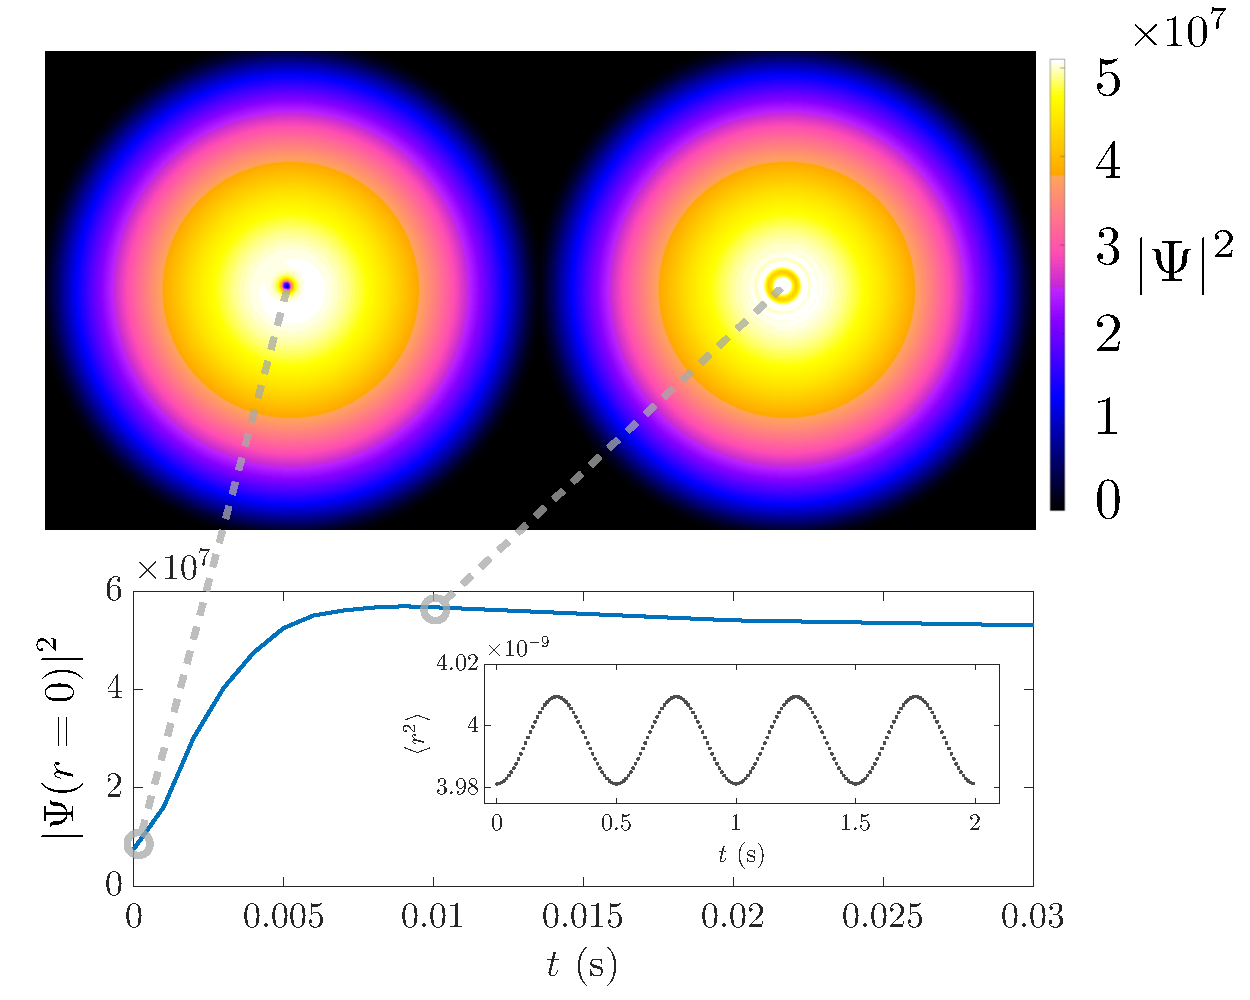
\includegraphics[width=0.7\textwidth]{ch6_phasegineer/arxiv/fig1.pdf}
    \caption{The evolution of the condensate density is shown for the initial state, and after 10 ms of evolution. The removal of the phase singularity at $t=0$ leads to a filling in of the density dip, which can also be seen from the line-plot (the singularity is initially located at $r=0$). The process excites the monopole mode at frequency $2\omega_\perp$ (see inset).}\label{fig:annihilation_1vtx}
\end{figure}
\begin{figure}\centering
    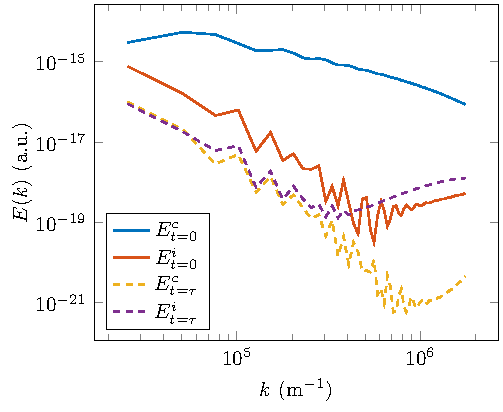
\includegraphics[width=0.6\textwidth]{ch6_phasegineer/tikz/EKt.pdf}
    \caption{Ratio of incompressible to compressible energy at  $t=0$ (solid) and $t=10$ ms (dashed). Initially the incompressible energy is greater than the compressible due to the presence of the vortex, giving values greater than unity for all $k$. After application of the phase profile, the vortex is annihilated, with the energy released as phonons, indicated by a decrease in incompressible energy for all $k$ values.}\label{fig:kinspec}
\end{figure}

While the above example suggests that erasing vortices is a straightforward and controllable process, this assumption must be checked for the situation where the imprinted phase singularity and the existing phase are not perfectly centered on each other. This is shown in Fig.~\ref{fig:annihilation_1vtx_uncentred}, and one finds that cases where the imprinted profile is sufficiently close to the core (i.e.\ within twice the healing length, $\xi\approx1.06\times 10^{-6}$ m) the existing vortex gets erased as before. However, beyond this distance a separate antivortex gets created and the vortex-antivortex pair travels to the edge of the condensate system and begins to circulate around~\cite{VTX:Martikainen_pra_2001}, as is shown in Sec.~\ref{sec:fewvtx}. For a densely packed lattice of vortices, however, this is not a problem as the typical distance between vortices is of comparable size with the healing length.

\begin{figure}\centering
    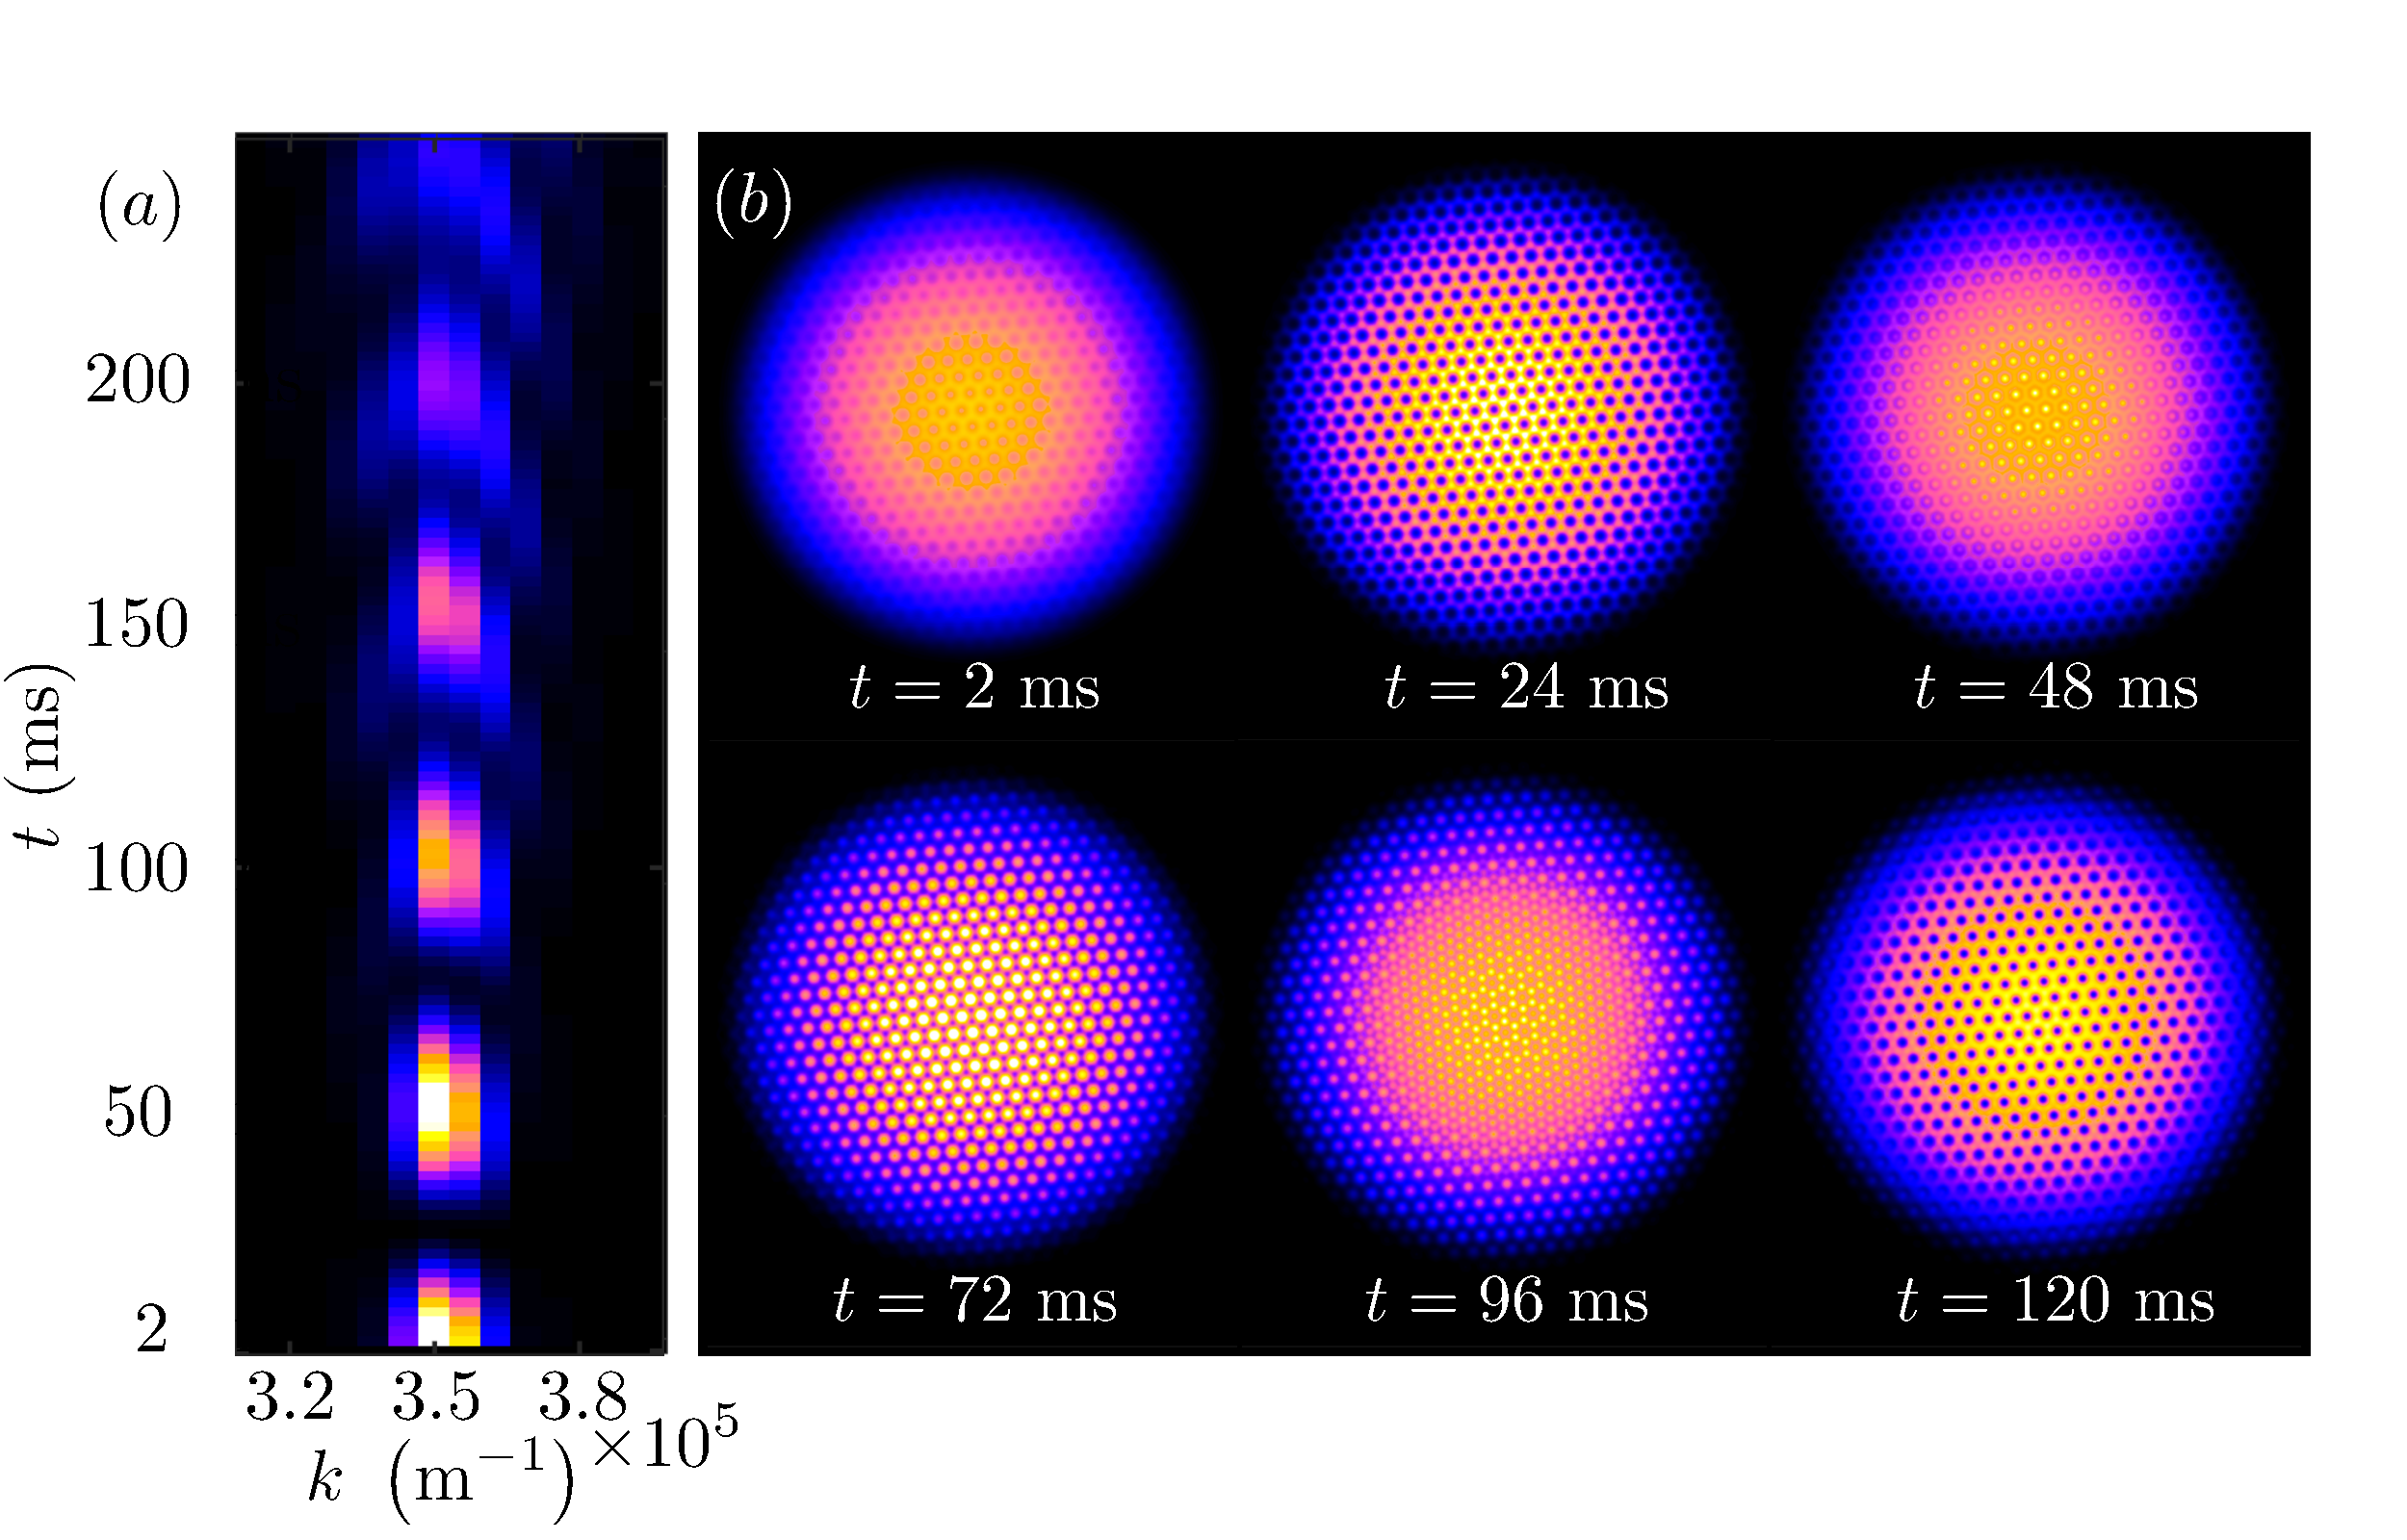
\includegraphics[width=0.7\textwidth]{ch6_phasegineer/arxiv/fig3.pdf}
    \caption{The condensate evolution following an uncentered phase imprint. For an imprint where the singularities of the vortex and the imprinted phase are less than a healing length away from each other, the existing vortex is annihilated and phonon modes are excited $(a,b)$. However, beyond this distance an antivortex is created, which travels with the pre-existing vortex and circulates the condensate $(c,d,e)$. The distance for cases $(a,b)$ and $(c,d,e)$ are $r = 1.36\times10^{-6}$ m, and $r =2.73 \times10^{-6}$ m respectively.}\label{fig:annihilation_1vtx_uncentred}
\end{figure}


\subsection{Lattice dynamics}

%%%%%%%%%%%%%%%%%%%%%%%%%%%%%%%%%%%%%%%%%%%%%%%%%%%%%%%%%%%%%%%%%%%%%%%%%%%%%%%%%%%%%%%%%%%%%%%%%%%%%%%%%%%%%%%%%%%%%%%%%%%%%%%%%%%%%%%%%%%%%

The removal of a single vortex from the vortex lattice by phase erasing initially affects only the nearest neighbours, as the phase gradient is only significant over the length scale of a healing length close to the erased singularity. The altered velocity profile will lead to the remaining vortices leaving their initial equilibrium positions in the Abrikosov lattice and the excitation of phonon modes. However, in the lattice areas away from the impurity, these phonon modes have only minimal impact on the geometry, as was observed with the optical lattice kicking described in Sec.~\ref{sec:moire_dyn_lattice}. To characterize the vortex dynamics following the application of the phase profile, we will in the following track each individual vortex throughout the full time-evolution and use the resulting trajectories, Delaunay triangulations, and Voronoi tessellations for analysis.

\begin{figure}\centering
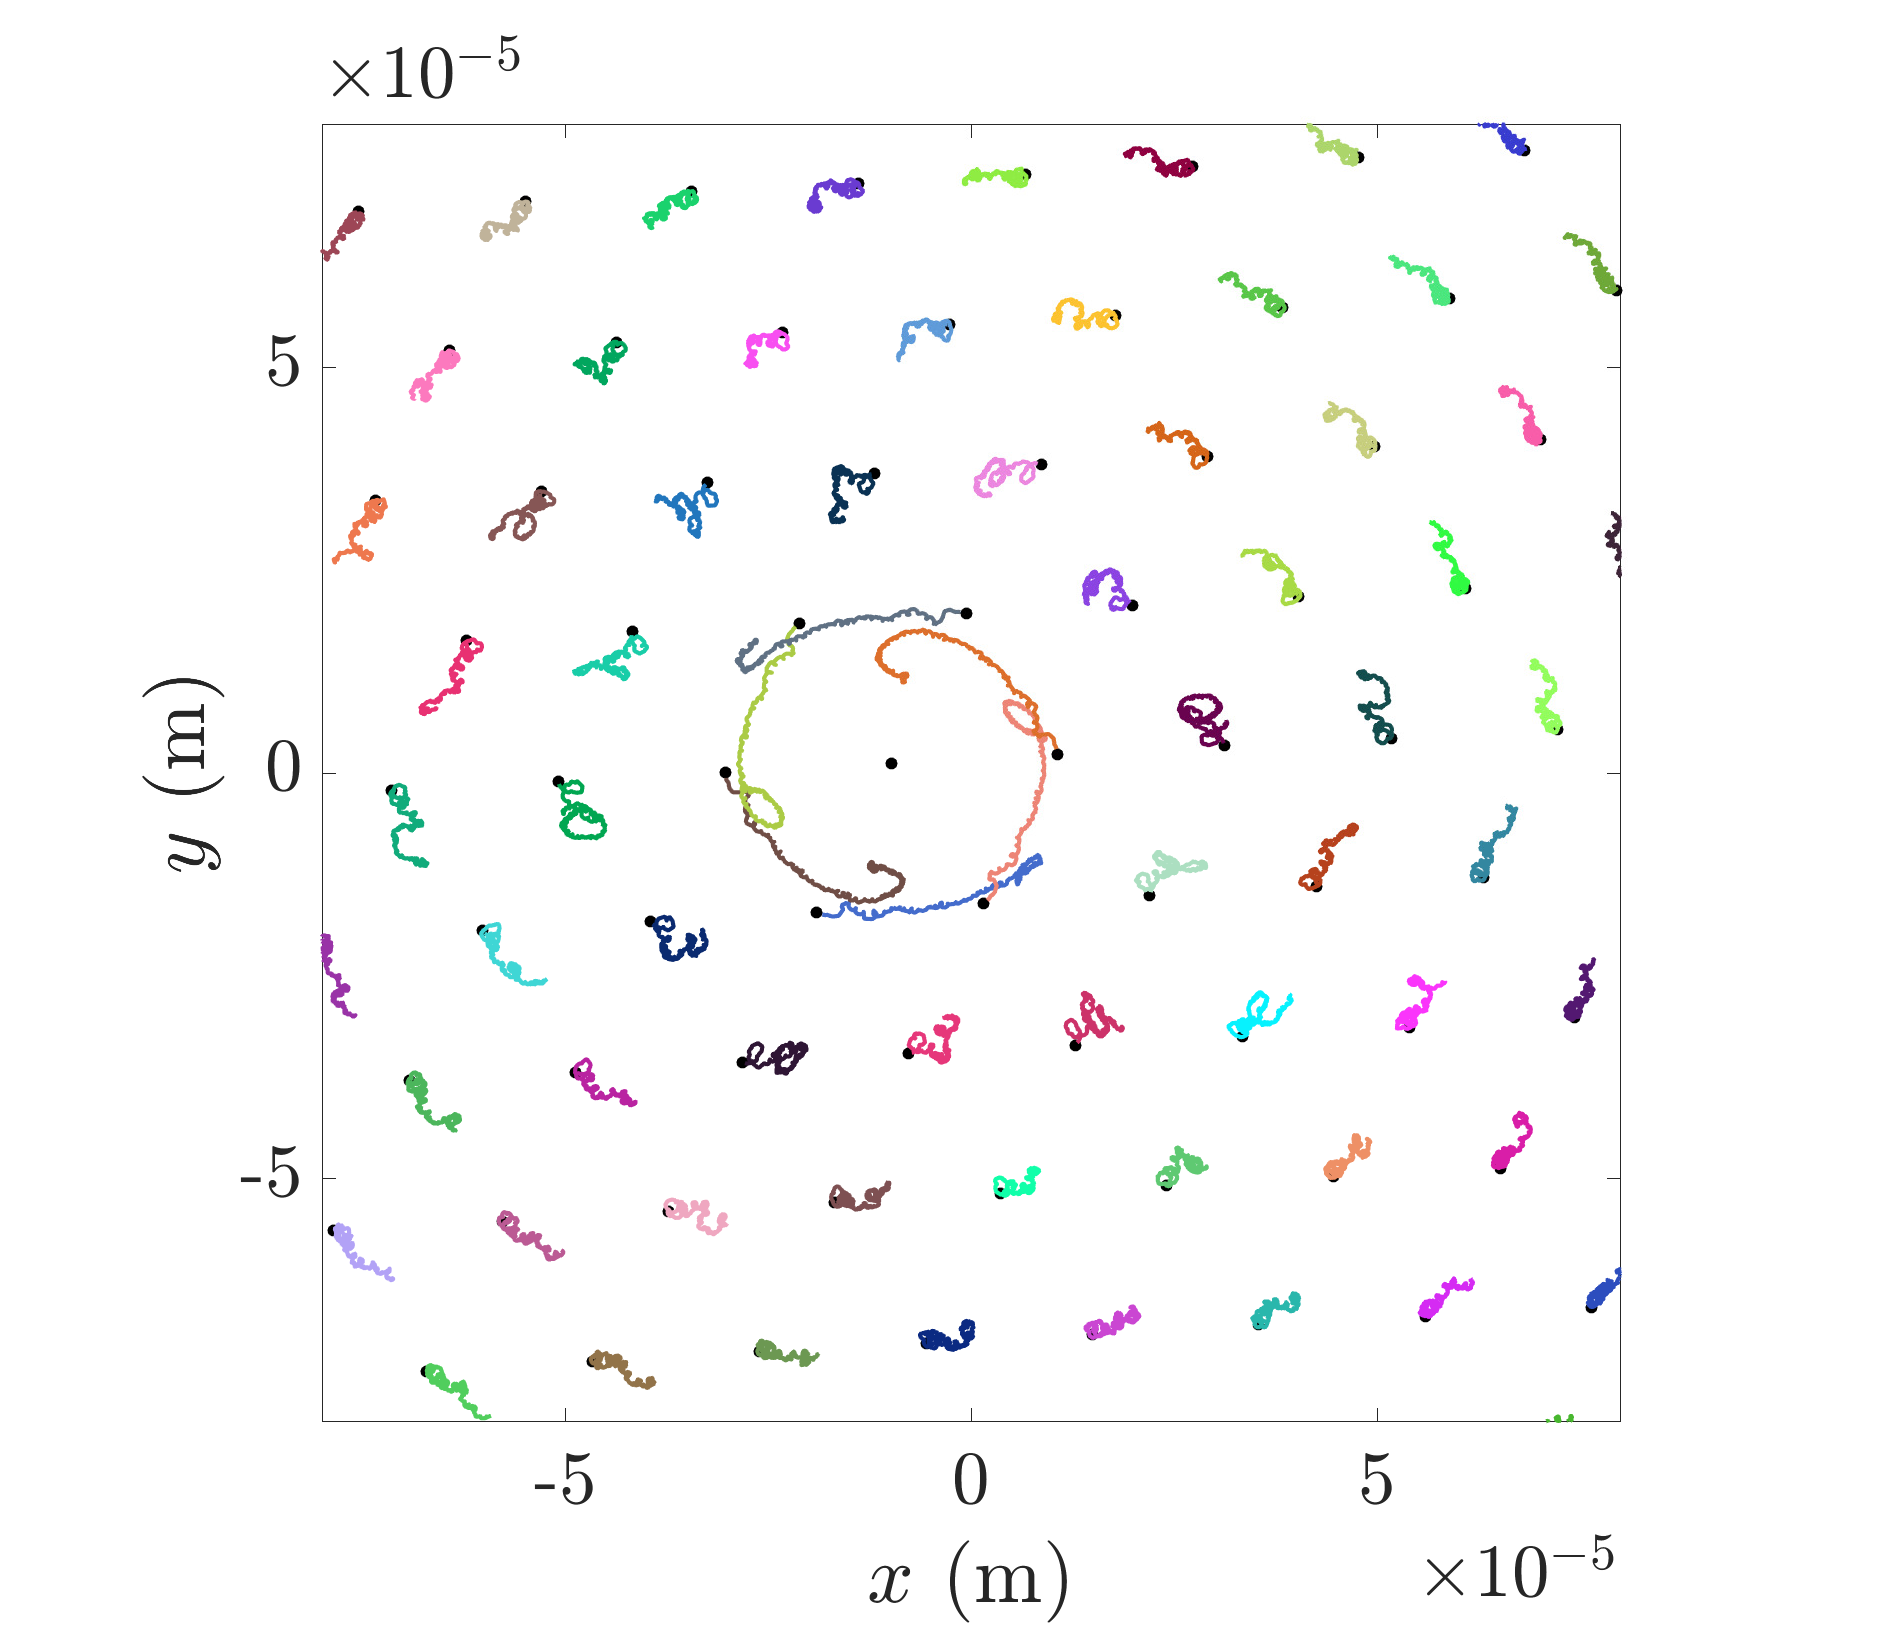
\includegraphics[width=0.7\textwidth]{ch6_phasegineer/arxiv/fig4.pdf}
    \caption{The trajectories of the vortices over 4 seconds (dt=$10^{-5}$, steps=$4\times 10^{5}$) following the removal of the vortex closest to the center, where each color represents a unique trajectory path, and black dots indicate positions at $t=0$. The vortices can be seen to move counter-clockwise in the co-rotating frame due to the loss of the local velocity field. However, the effect of the removal decreases quickly with increased radial distance. }
    \label{fig:trajplot}
\end{figure}


\begin{figure}\centering
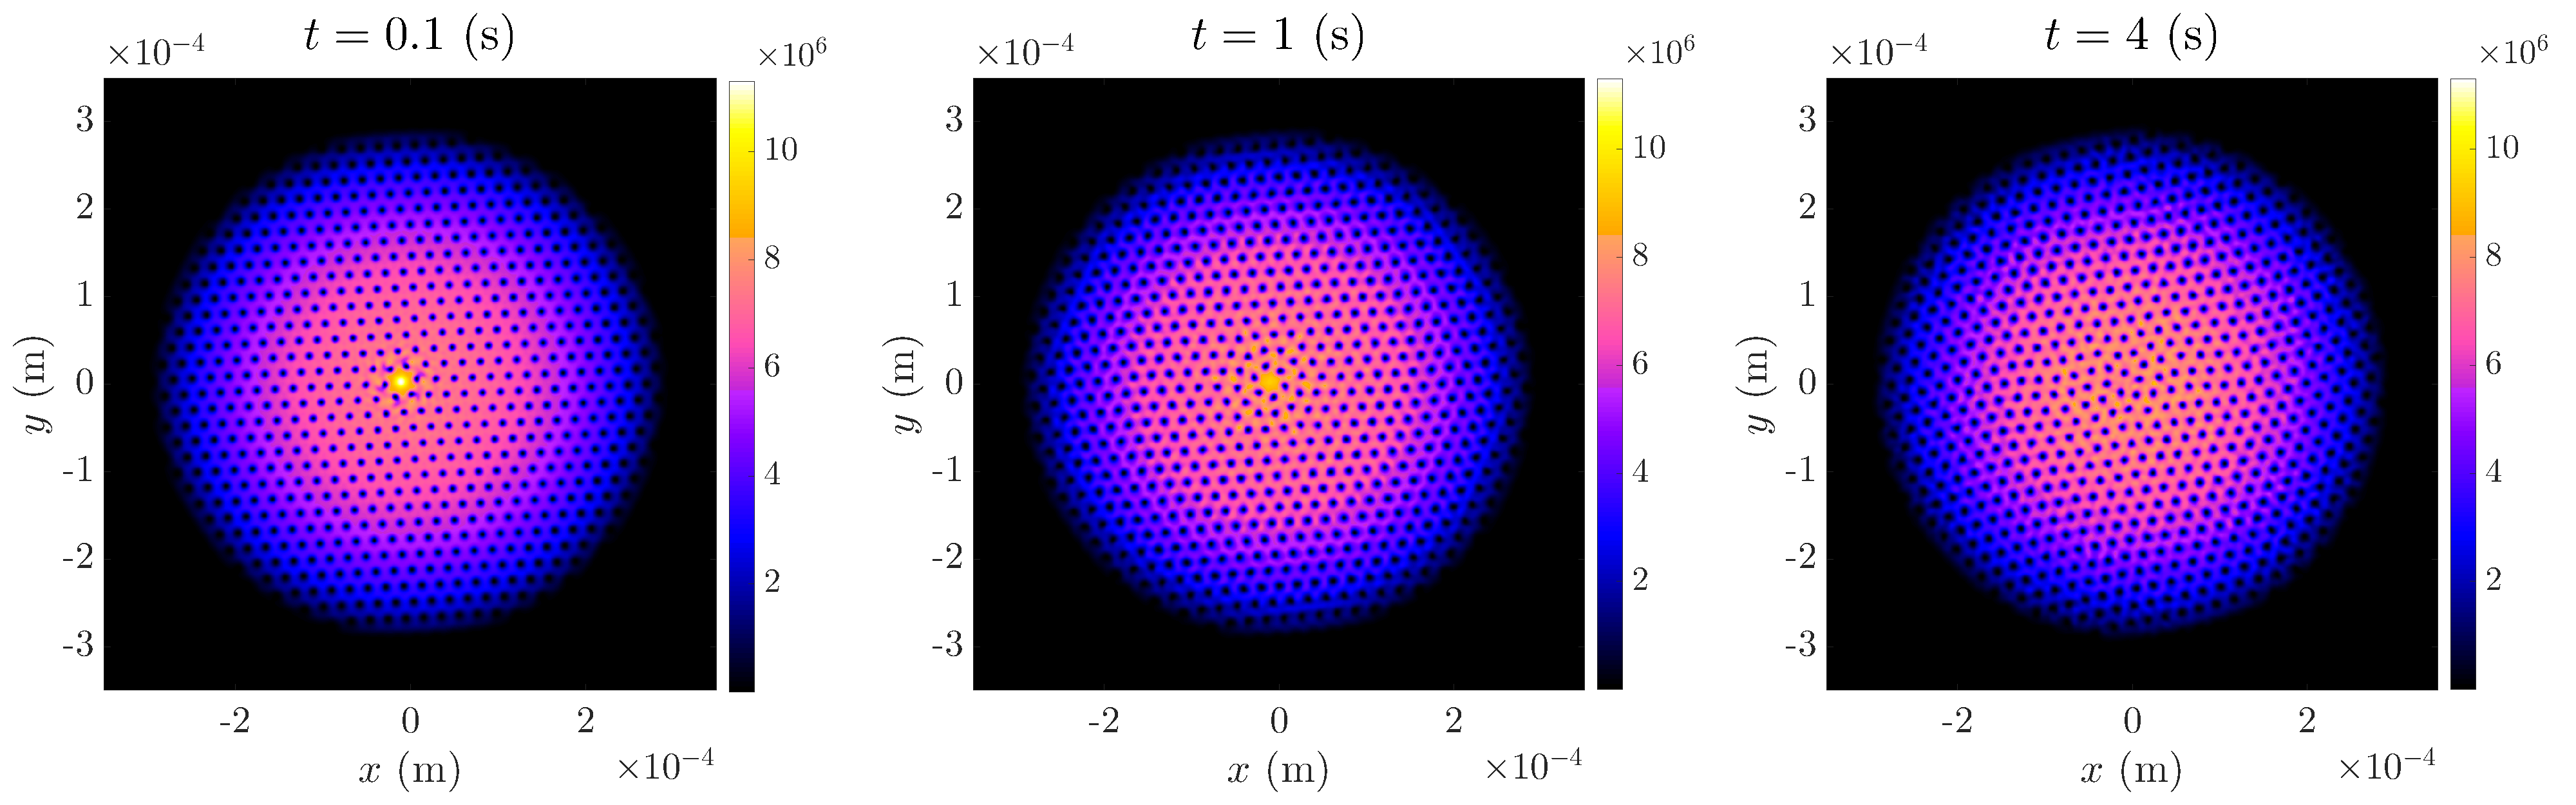
\includegraphics[width=0.96\textwidth]{ch6_phasegineer/varr_161_rho}
    \caption{ Wavefunction densities following a vortex removal close to the centre of the condensate. The vacancy region exists for some time after the removal, before the honeycomb-like structure decays and locally disorders the vortex lattice. }
    \label{fig:varr161_rho}
\end{figure}
Let us first consider the situation where a single vortex is erased within the central area of the vortex lattice. In Fig.~\ref{fig:trajplot} we show the trajectories of the remaining vortices over a time-scale of 4 seconds, and the corresponding wavefunction densities at $t=(0.1,1,4)$ s in Fig.~\ref{fig:varr161_rho}. One can see that a long-lived vacancy is maintained close to the centre with the adjacent vortices rotating faster than the lattice due to the loss of the local velocity field. The honeycomb-like vacancy region eventually decays and the system settles into a new local geometry. The velocity field magnitude and direction of the condensate local to the removal site are shown in Fig.~\ref{fig:varr161_velfield} for $t=(0.01,0.1)$ s. Almost directly following the imprint, the removal site shows a phononic flow that fills in the now unstable dip in the density, and which eventually disperses across the lattice. The small-scale flow magnitude that exists in the remaining region is sufficient to allow for the decay of the honeycomb-like structure during the subsequent time evolution.

\begin{figure}\centering
    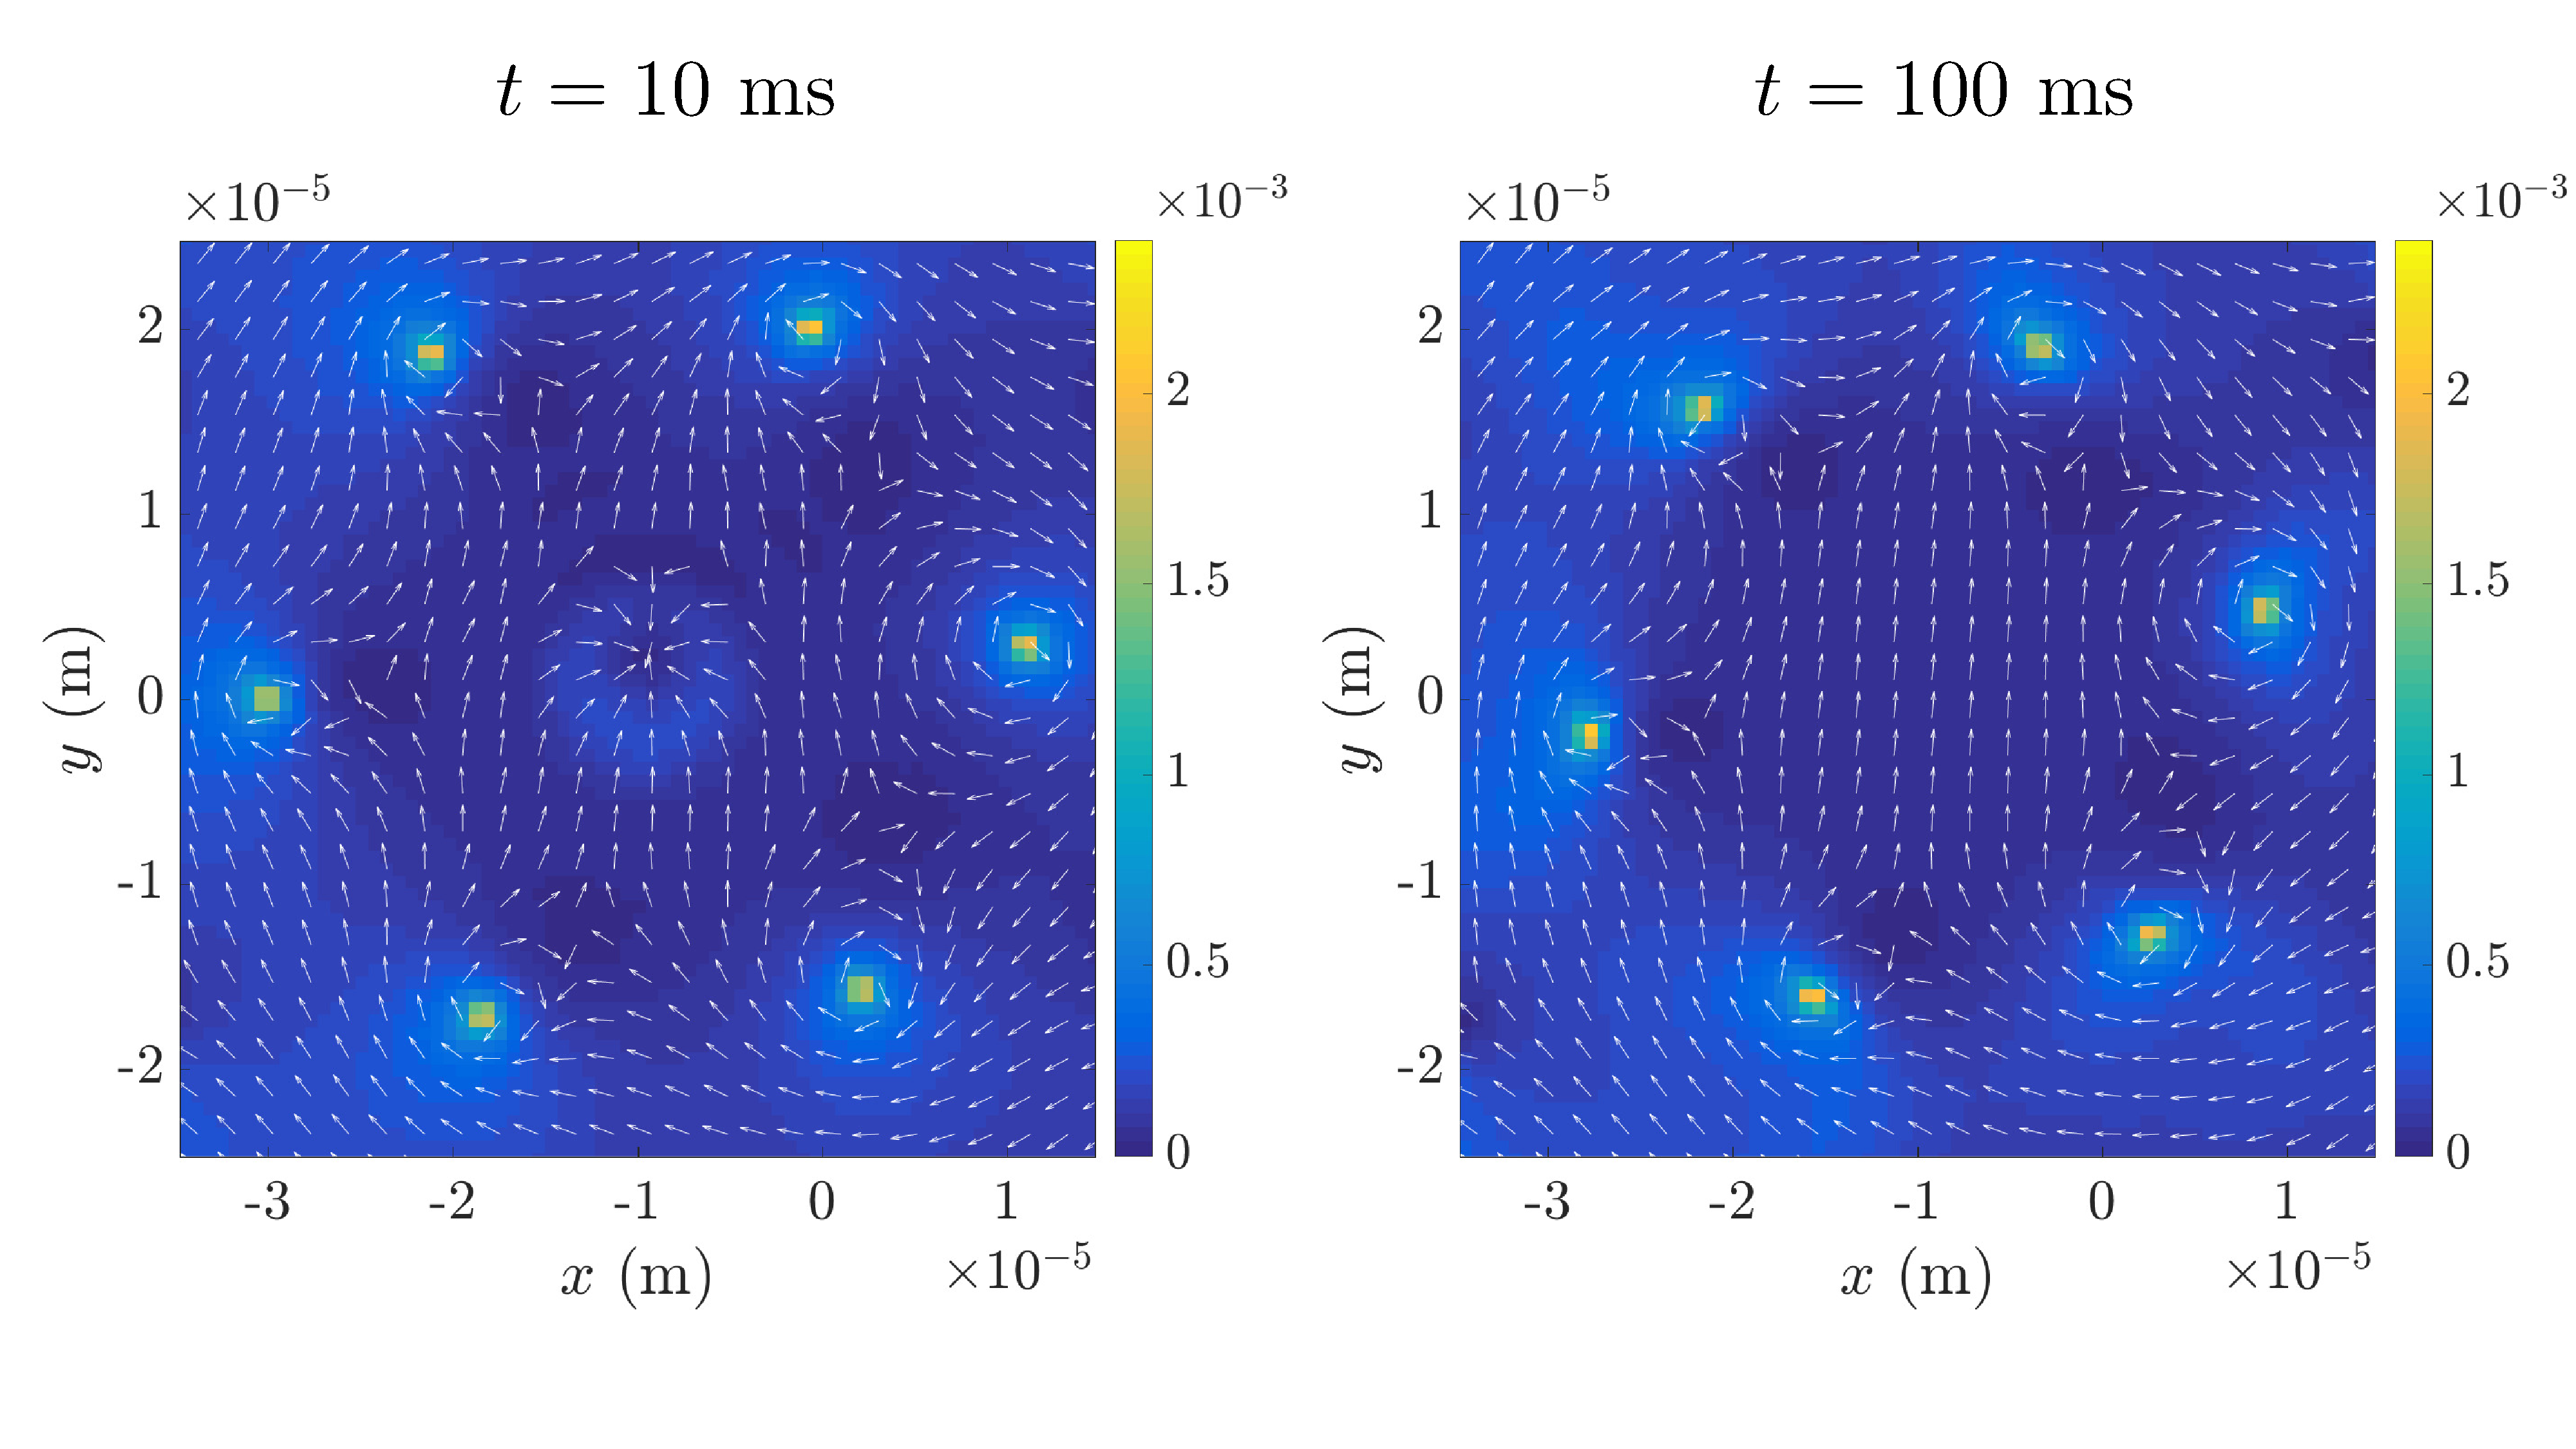
\includegraphics[width=0.95\textwidth]{ch6_phasegineer/velfield/var161_velfield}
    \caption{The velocity field magnitude and direction following the removal of a centrally located vortex from the lattice. At $t=10$ ms a phononic flow can be observed, resulting from the vortex annihilation. For $t=100$ ms, a net flow across the previous position of the erased vortex indicates an instability in the region, eventually leading to decay of the vacancy region. }\label{fig:varr161_velfield}
\end{figure}

Similar behavior can be observed if the erased vortex is not within the central area, as long as it is within a region of constant areal vortex density. However, being closer to the edge of the lattice reduces the stability of the perturbed region, which is likely due in part to the solid-body velocity field of the vortex lattice away from the centre. The overall lattice remains well structured after a vortex removal, as can be seen from the orientational correlation function shown in Fig.~\ref{fig:g6} for different times. Although the gaps between the peaks that exist at $t=0$ disappear during the evolution due to the presence of the phonon excitation, the overall correlations remain high for long times and near constant across all length scales. The slight peak softening arises from the vortices no longer being aligned to a perfect triangular lattice position, which is indicative of a weak disordering or distortion of the lattice structure.

\begin{figure}\centering
    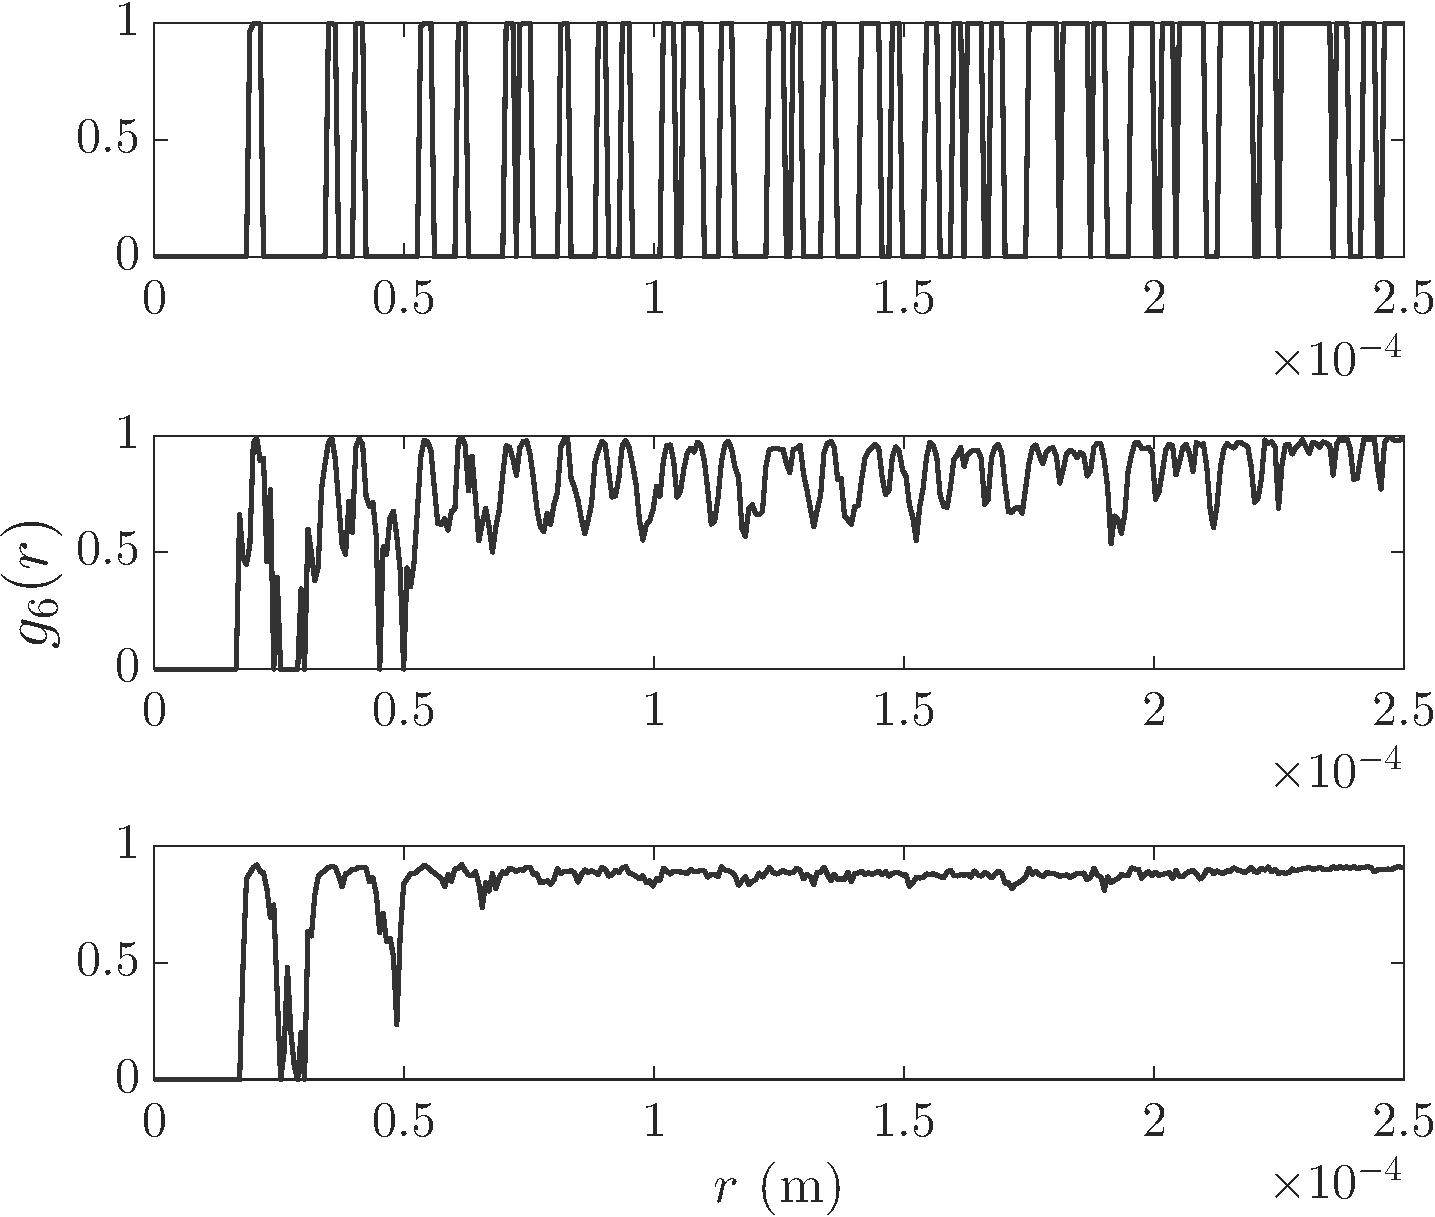
\includegraphics[width=0.6\textwidth]{ch6_phasegineer/arxiv/fig5.pdf}
    \caption{The orientational correlation function for the vortex lattice after removing the central vortex is given for $t=(0,1,6)$ seconds (top to bottom). The peaks at $t=0$ appear at nearest neighbour, next nearest, and higher order distances. Due to finite binning of the lengths, the peaks become grouped to 1 at higher length scales. For times greater than $t=0$ the peak correlations drop, however, the large value at long times indicates a well ordered lattice as high correlations are observed across all length scales.}\label{fig:g6}
\end{figure}

As described above, the Delaunay triangulation of the lattice can give a graphical overview of how connected the different vortices are, and therefore what changes to the lattice structure have occurred \cite{Guillamon_nat_2014}. We show the case where a single vortex was removed from the lattice centre in Fig.~\ref{fig:deltri_1vtx}. One can see that a pair of (5,7)-fold connected lattice defects have formed after the removal (at 10 ms), which slightly adjusts and becomes stable for longer times. Removing vortices at different positions in the lattice shows similar behavior, with a localization of the disordered region not far from the site of the vortex removal.

\begin{figure}\centering
    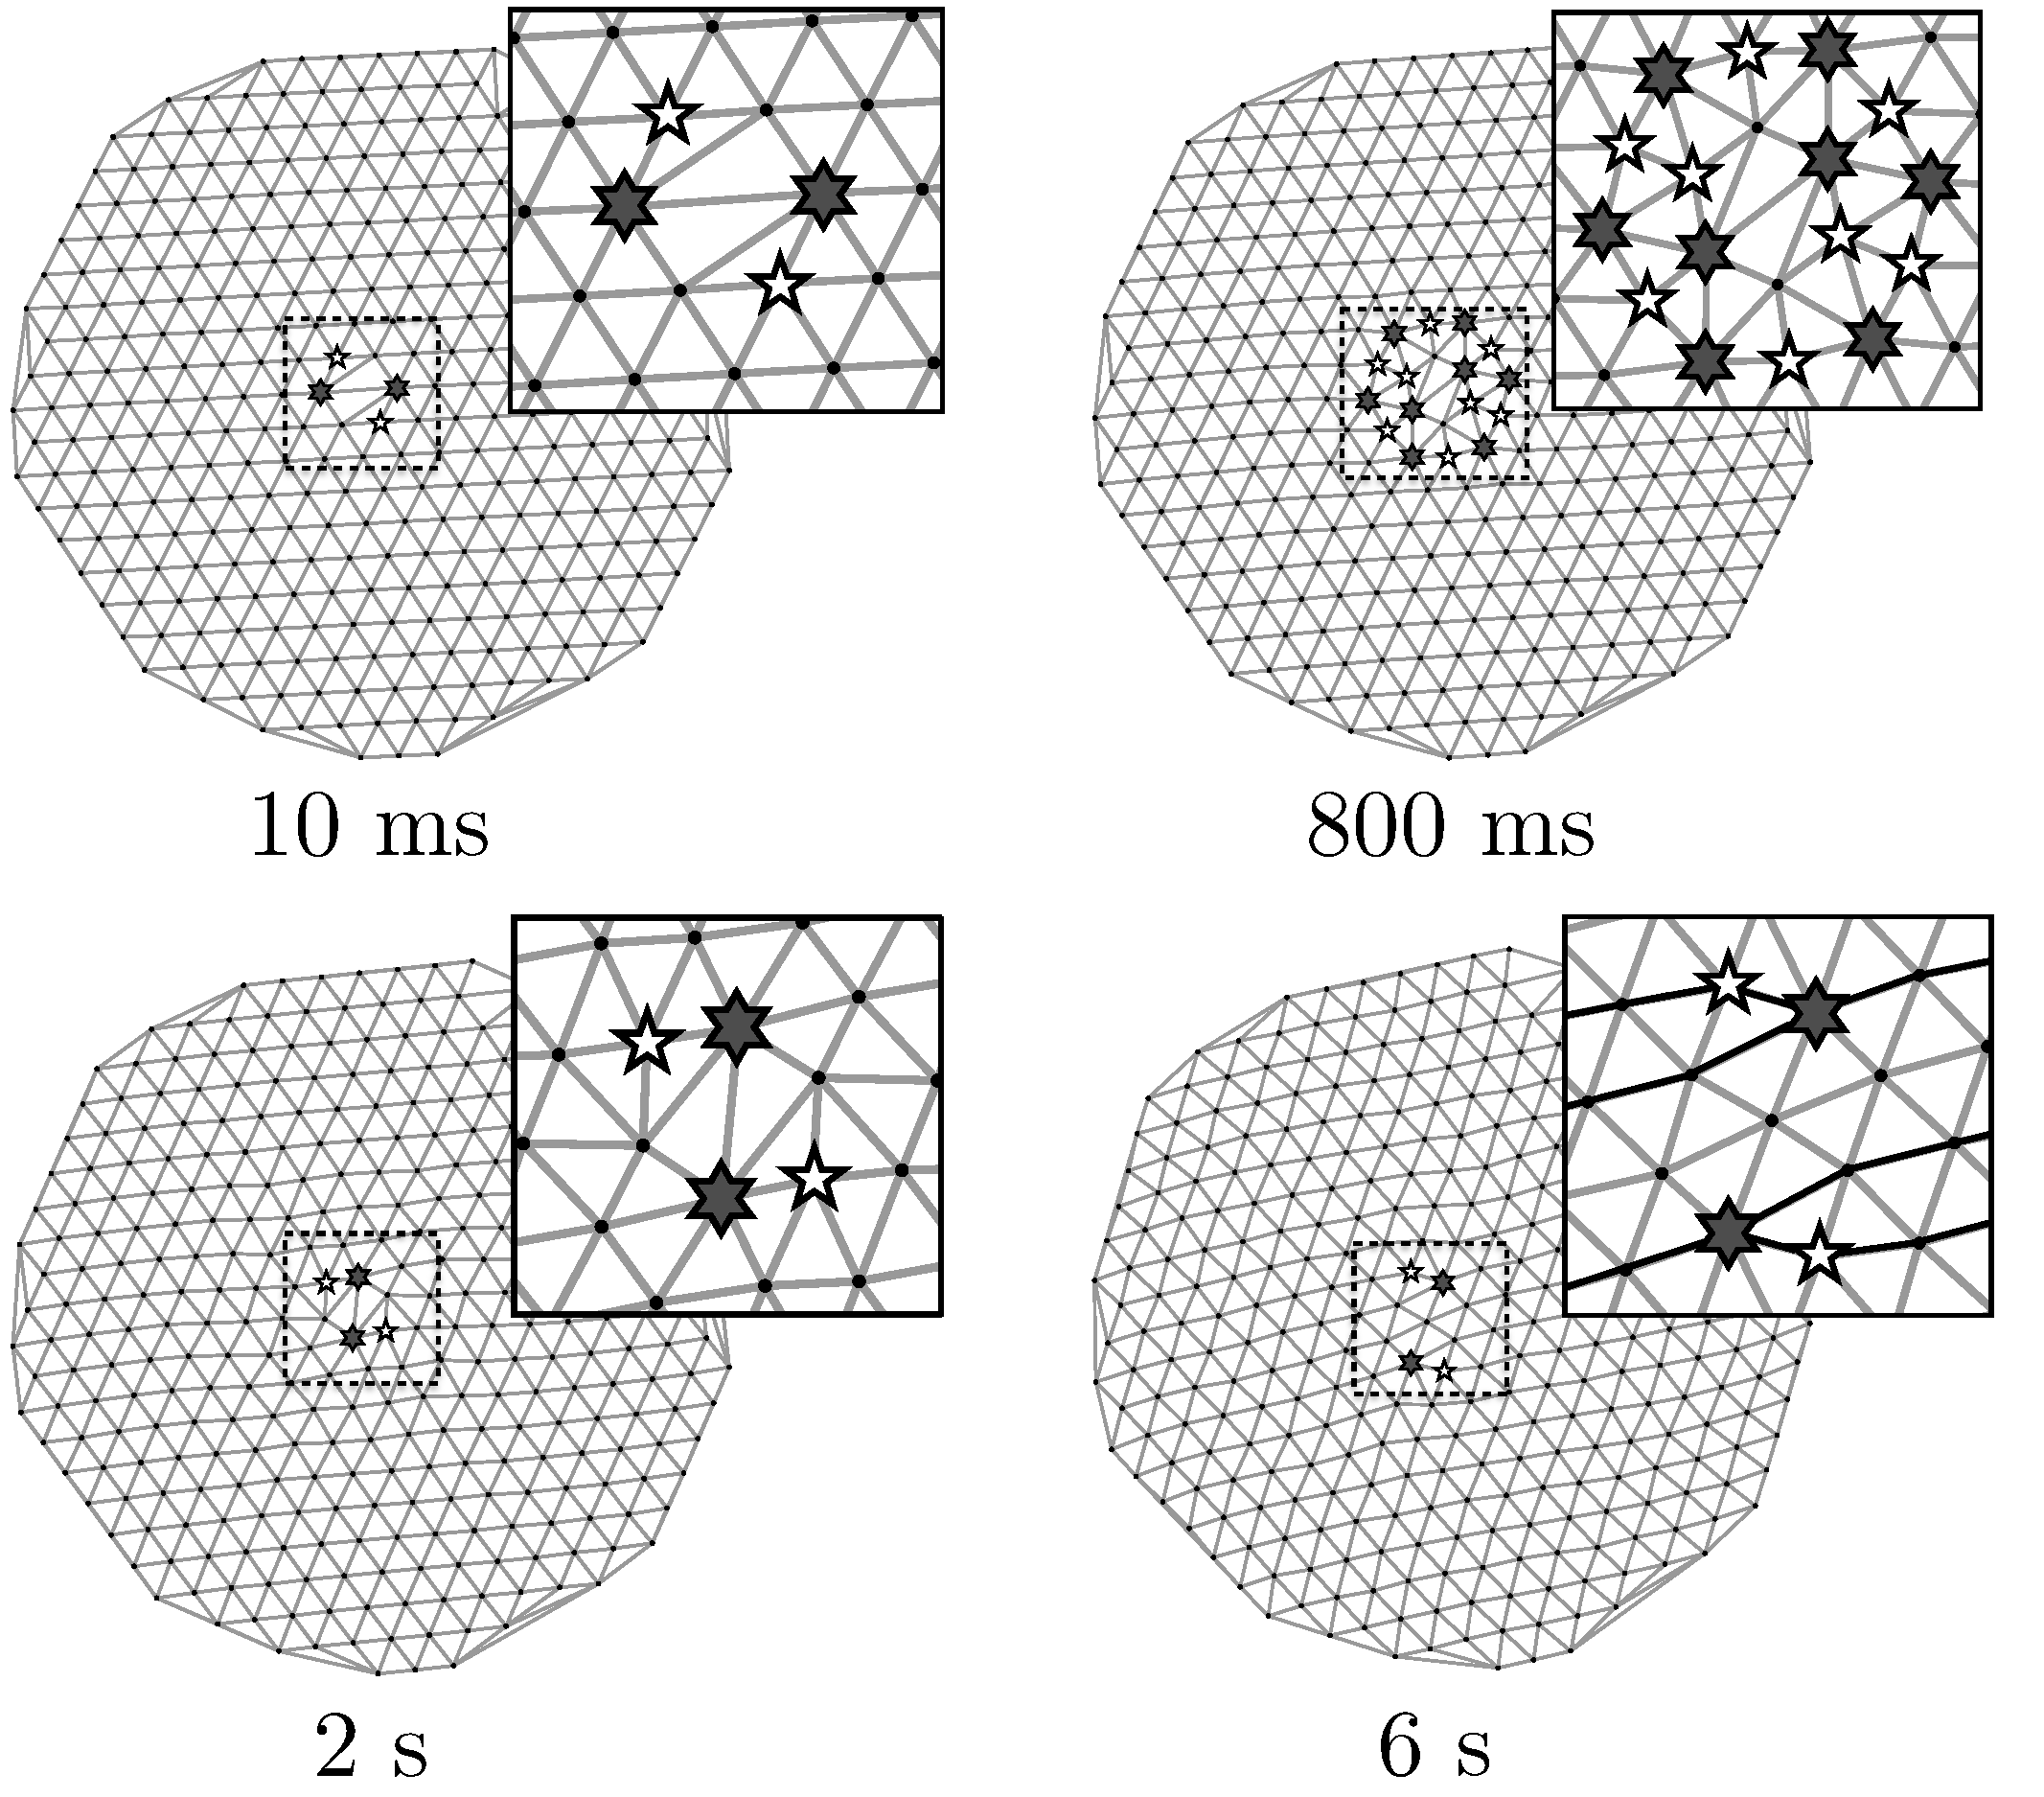
\includegraphics[width=0.7\textwidth]{ch6_phasegineer/arxiv/fig6.pdf}
    \caption{Delaunay triangulation of the vortex lattice after removing one vortex, shown at $t=(0.01,0.8,2,6)$ s. The resulting lattice defects are indicated by white and gray stars for 5-fold and 7-fold defects respectively. One can see that two (5,7) dislocations are formed quickly, which settle and persist in the lattice for long times. Lattice dislocation lines are indicated as black lines for inset $t=6$ s.}\label{fig:deltri_1vtx}
\end{figure}

If the phase imprinting is not directly aligned with the vortex singularity, other $n$-fold dislocations can be found in the Delaunay triangulation. This is due in part to the vortex core size becoming comparable to the average spacing between the vortices in rapidly rotating condensates, and therefore the imprinted changes to the velocity field affect more nearby vortices. To investigate this effect at the lattice centre, a series of simulations were performed by imprinting at different locations as a function of $r$ and $\theta$. Due to the lattice symmetry, the resulting dynamics can be completely obtained by examining the region of $r=[0,a_v/2)$ and $\theta=[0,\pi/6)$. A schematic of this shown in Fig.~\ref{fig:hex}.

\begin{figure}\centering
    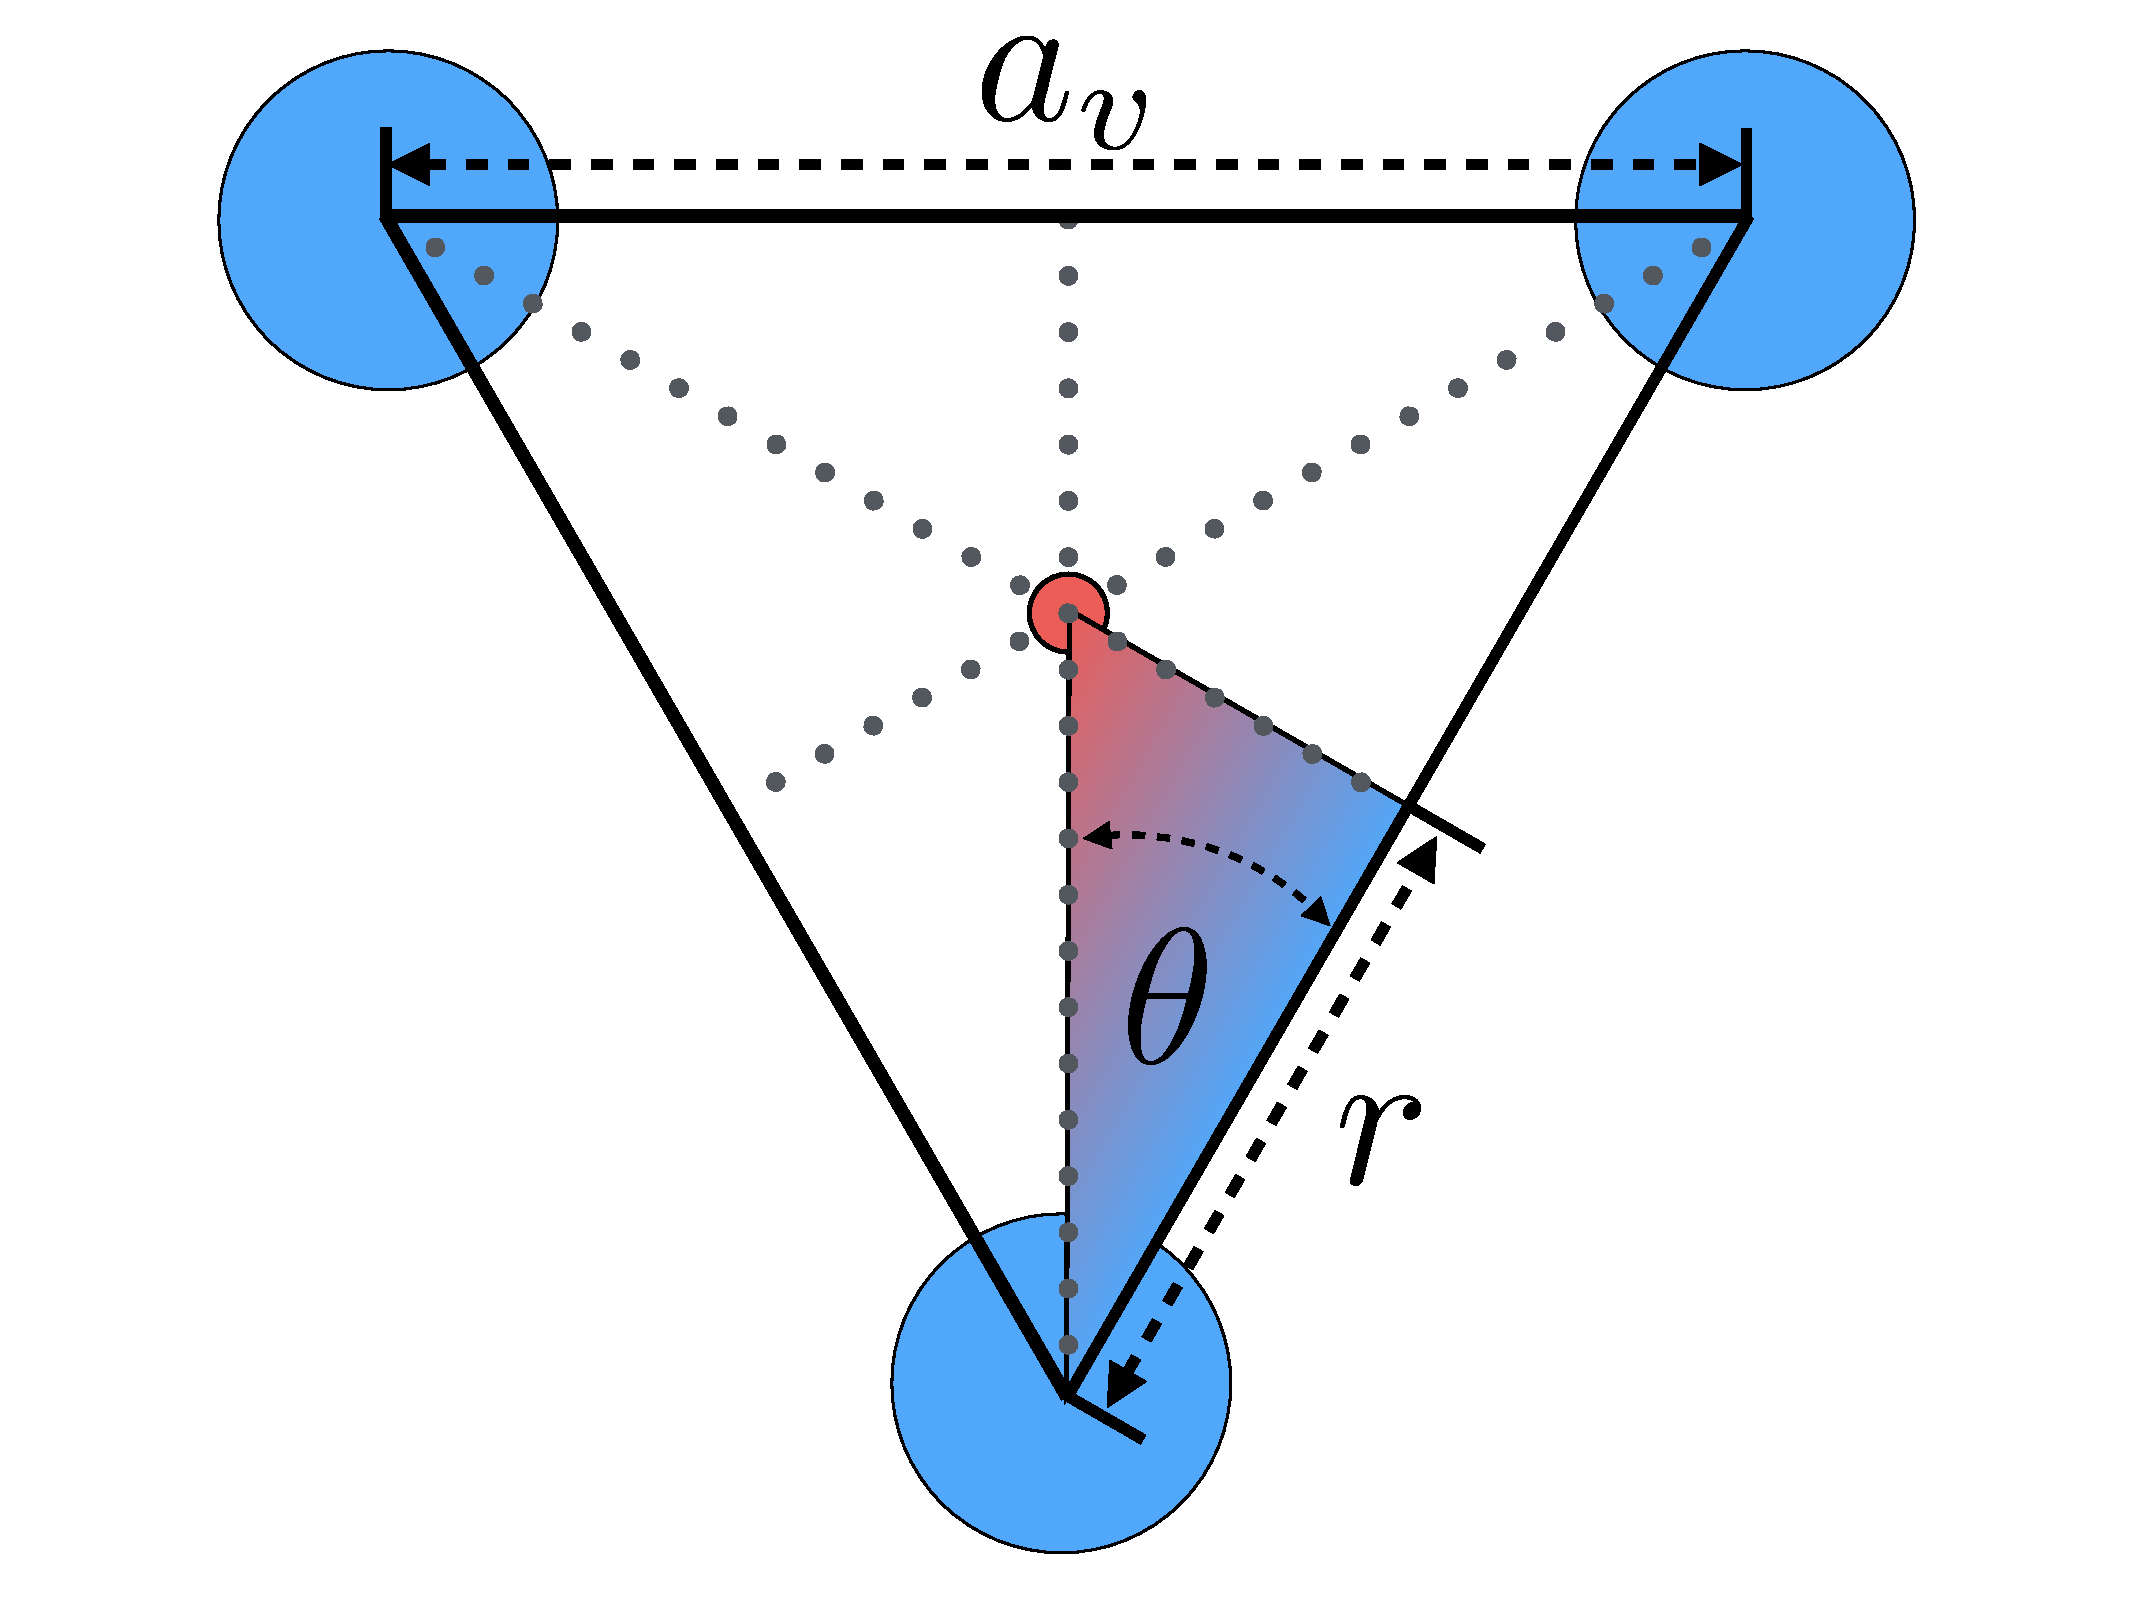
\includegraphics[width=0.5\textwidth]{ch6_phasegineer/hex.pdf}
    \caption{Schematic of triangular cell of the vortices. Due to the symmetry of the cell, an imprint within the shaded region can allow for all of the resulting dynamics to be determined.} \label{fig:hex}
\end{figure}

Figure~\ref{fig:lattice_misalign} shows the time-averaged number of lattice defects following the imprint within this examined region. One can see that if the displacement is still within the core of the vortex, on average 1 or 2 defects are created of the 5-fold ($a$) and the 7-fold ($b$) kind. At $r\approx a_v/4$ from the core centre, the imprint tends to create upwards of 3 to 4 defects, which again tends back to the average of 2 beyond this region. This shows that the previously discussed issue resulting from the creation of antivortices through imperfect alignment does not exist in Abrikosov lattices, and we will concentrate on the perfect imprint of the phase in the following discussions.

\begin{figure}\centering
    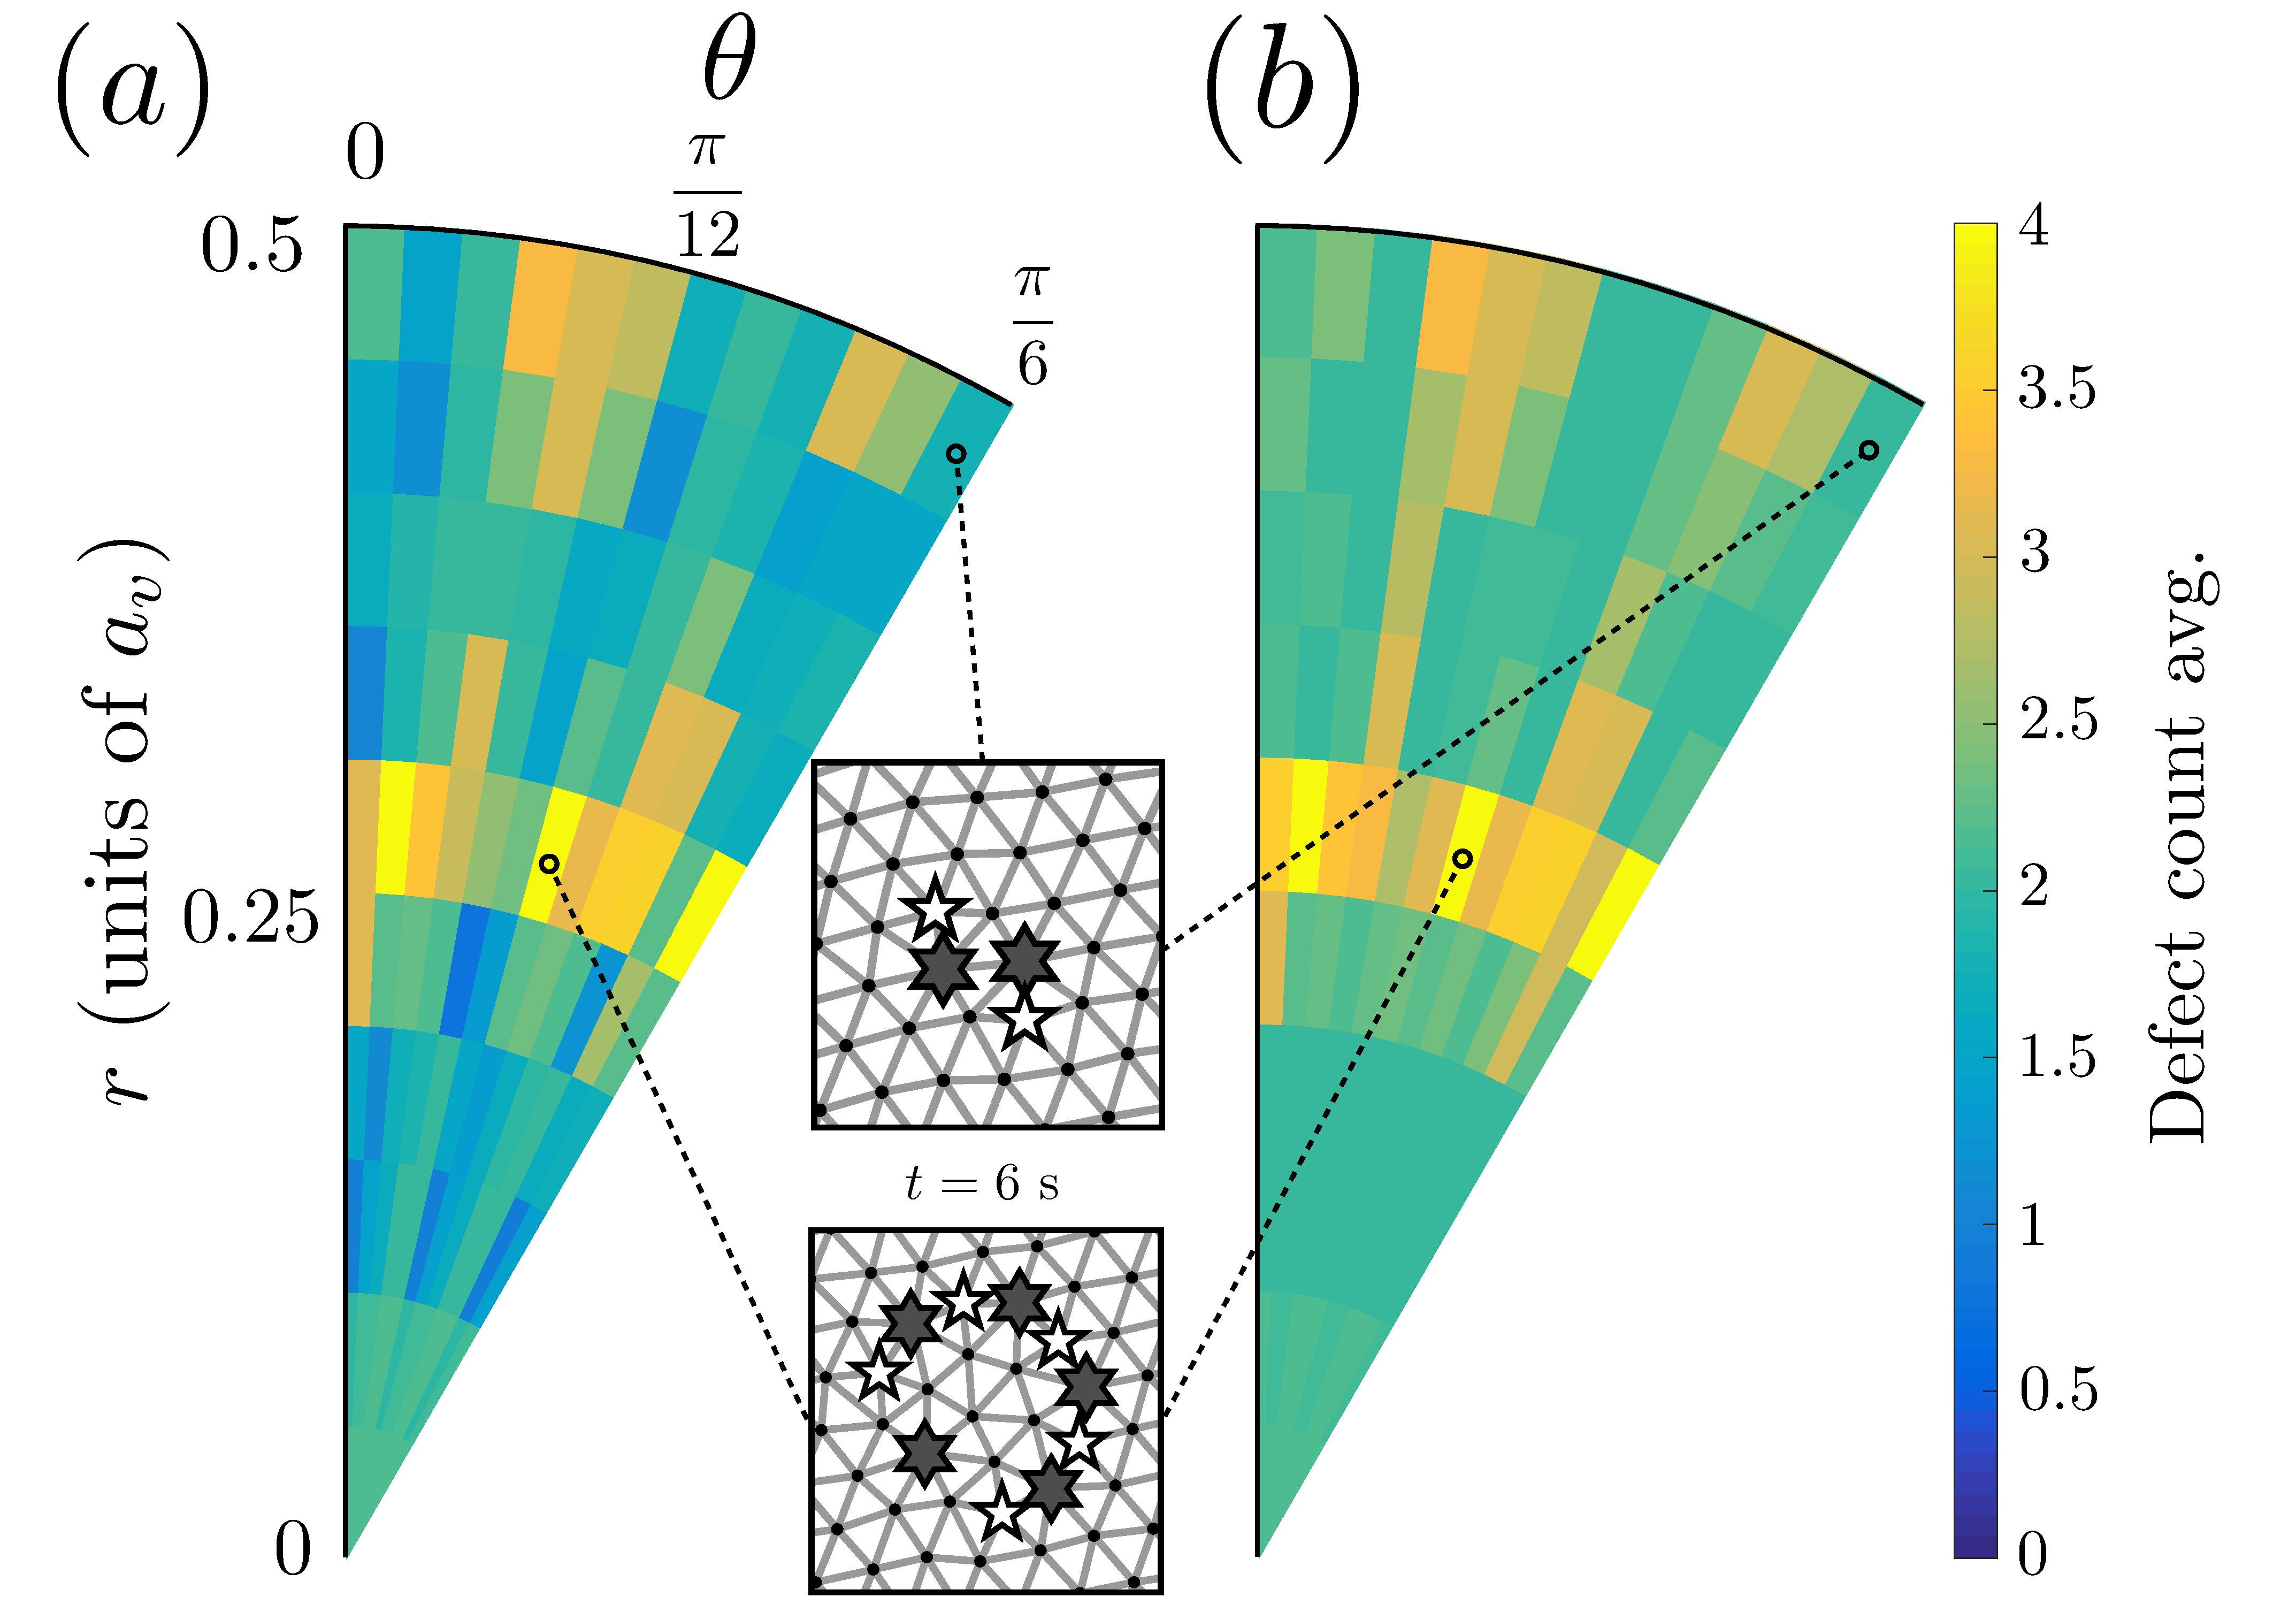
\includegraphics[width=0.7\textwidth]{ch6_phasegineer/arxiv/fig7.pdf}
    \caption{The time-averaged number of defects appearing over a range of imprint positions, relative to a central vortex from $t=1\rightarrow$10 s, and allowing 1 s of settling time. Both 5-fold ($a$) and 7-fold ($b$) defects are shown. The insets show a snapshot of two different parameter regions at $t=6$ s. A high simultaneity is observed between their appearance, where a paired (5,7) defect indicates a lattice dislocation. However, not all 5 and 7-fold defects pair, as some can exist individually, or pair with other $n$-fold defects.} \label{fig:lattice_misalign}
\end{figure}

To further demonstrate the localized nature of the defects, let us briefly discuss the situation where two vortices are erased in separate regions away from the lattice centre. The Delaunay triangulation for this case is shown in Fig.~\ref{fig:traj_2vtx_edge}, and the independence of the two localized regions is clearly visible, with each showing behavior similar to the case discussed above. Since we are limiting ourselves here to perfect imprinting, we also show the number of edges formed between vortices as a function of time for 5, 6 and 7 nearest neighbours respectively ($N_x$) in Fig.~\ref{fig:vtx_rem2_edge}. One can see that the initial perturbation settles quickly to values similar to the ones above.

\begin{figure}\centering
    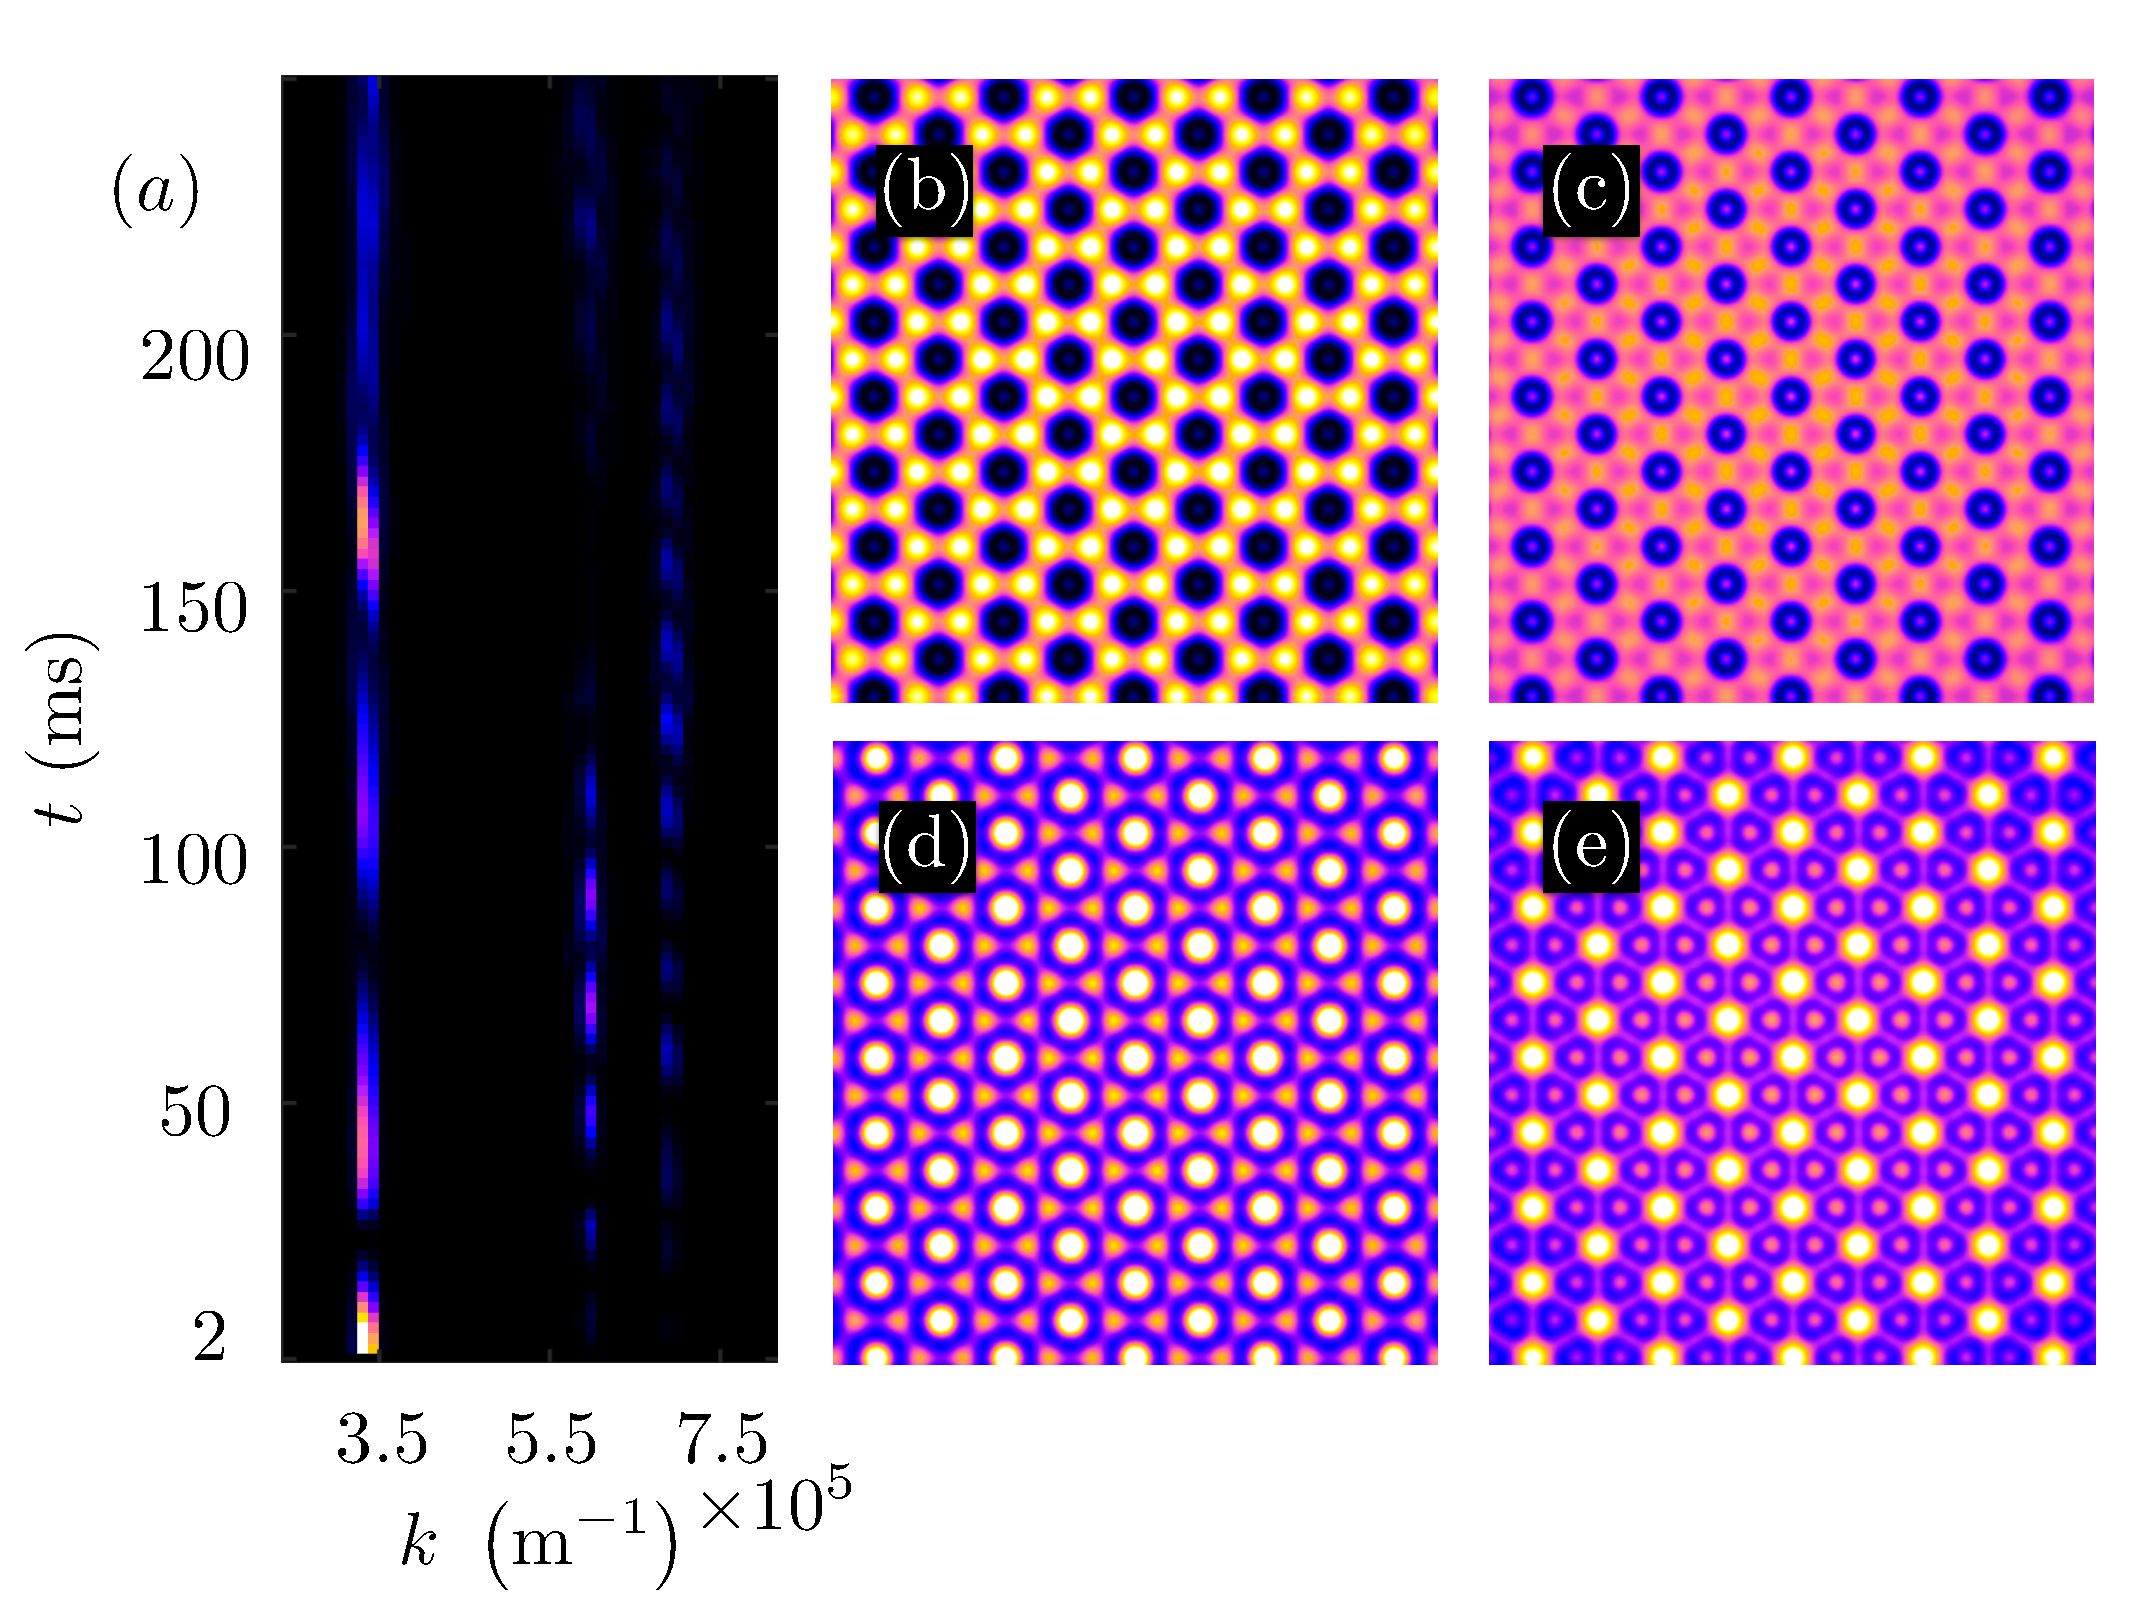
\includegraphics[width=0.6\textwidth]{ch6_phasegineer/arxiv/fig8.pdf}
    \caption{Delaunay triangulation of the vortex lattice upon removal of two vortices at either sides of the lattice for $t=(0.01,0.8,2,6)$ s. The resulting defects remain localized for long times and can therefore be considered independent. The lattice largely remains ordered, similar to the case of removing the central vortex discussed above. The appearance of an 8-fold connected vortex can also be observed at $t=0.8$ s (blue dot).}\label{fig:traj_2vtx_edge}
\end{figure}

\begin{figure}\centering
    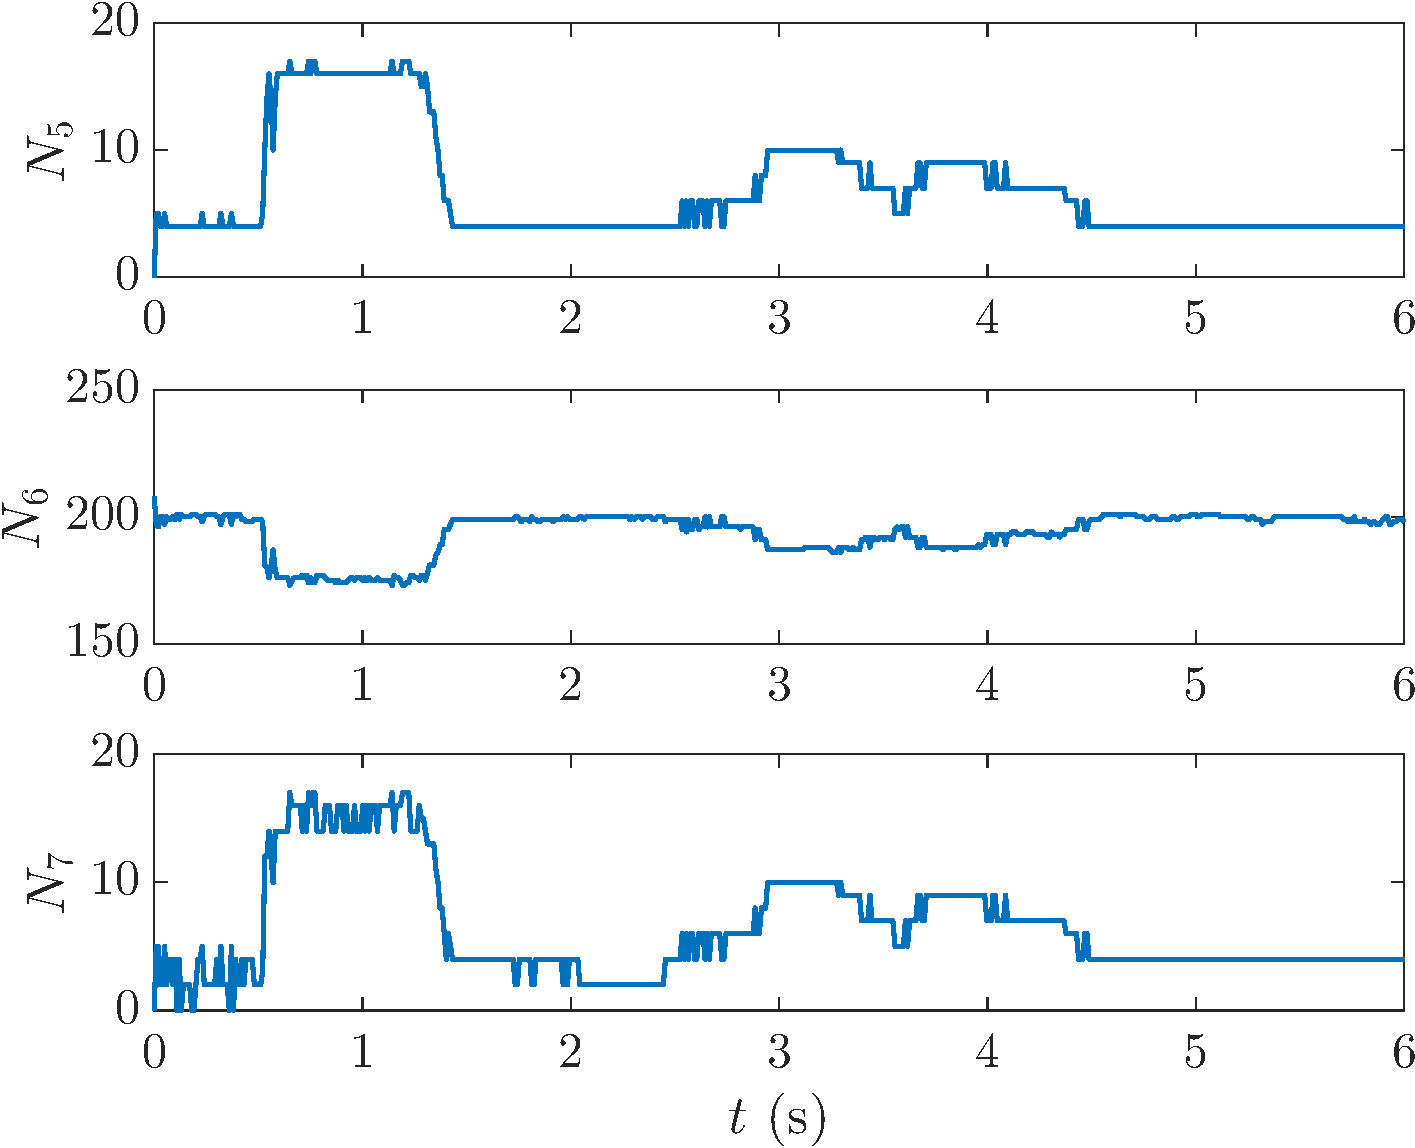
\includegraphics[width=0.5\textwidth]{ch6_phasegineer/arxiv/fig9.pdf}
    \caption{The defect ($N_5,~N_7$) and triangular lattice ($N_6$) nearest neighbour count taken from a Delaunay triangulation of the vortex lattice following the removal of two vortices on opposite sides as a function of time. After a brief settling time, the lattice attains an almost constant defect count.}
    \label{fig:vtx_rem2_edge}
\end{figure}

%%%%%%%%%%%%%%%%%%%%%%%%%%%%%%%%%%%%%%%%%%%%%%%%%%%%%%%%%%%%%%%%%%%%%%%%%%%%%%%%%%%%%%%%%%%%%%%%%%%%%%%%%%%%%%%%%%%%%%%%%%%%%%%%%%%%%%%%%%%%%
%%%%%%%%%%%%%%%%%%%%%%%%%%%%%%%%%%%%%%%%%%%%%%%%%%%%%%%%%%%%%%%%%%%%%%%%%%%%%%%%%%%%%%%%%%%%%%%%%%%%%%%%%%%%%%%%%%%%%%%%%%%%%%%%%%%%%%%%%%%%%

In addition to simply erasing vorticity, we can also use phase imprinting to create varying degrees of disorder. By, for example, applying an appropriate $4\pi$ magnitude phase imprint we can replace a vortex with an antivortex at a given position. Since this does not require a change in the local density, all resulting perturbations stem from the adjusted velocity field of the vortex that has been flipped~\cite{VTX:Madarassy_gfd_2009}, with snapshots at $t=(10,100)$ ms shown in Fig.~\ref{fig:varr161anti_velfield}. Here we can clearly see the change in velocity field direction around the central vortex relative to the surrounding vortices. This in turn causes the surrounding vortices to rotate at a different rate than the solid-body rate of the overall lattice, creating a loss of triangular symmetry in this region on a faster scale than removing a single vortex. It is immediately obvious that such a situation is unstable, which can be confirmed by observing the creation of a large number of defects during the evolution, as shown in Fig.~\ref{fig:varr161anti_defect}. An increase in the number of defects can be seen up to approximately $t=3$ s, during which the antivortex causes local disordering of the lattice, annihilates with a nearby vortex, and gives rise to the creation of a large number of (5,7) defect pairs. After this the number of defects no longer grows, but instead fluctuates about a stable value which is greater than that of the previously examined cases.

\begin{figure}\centering
    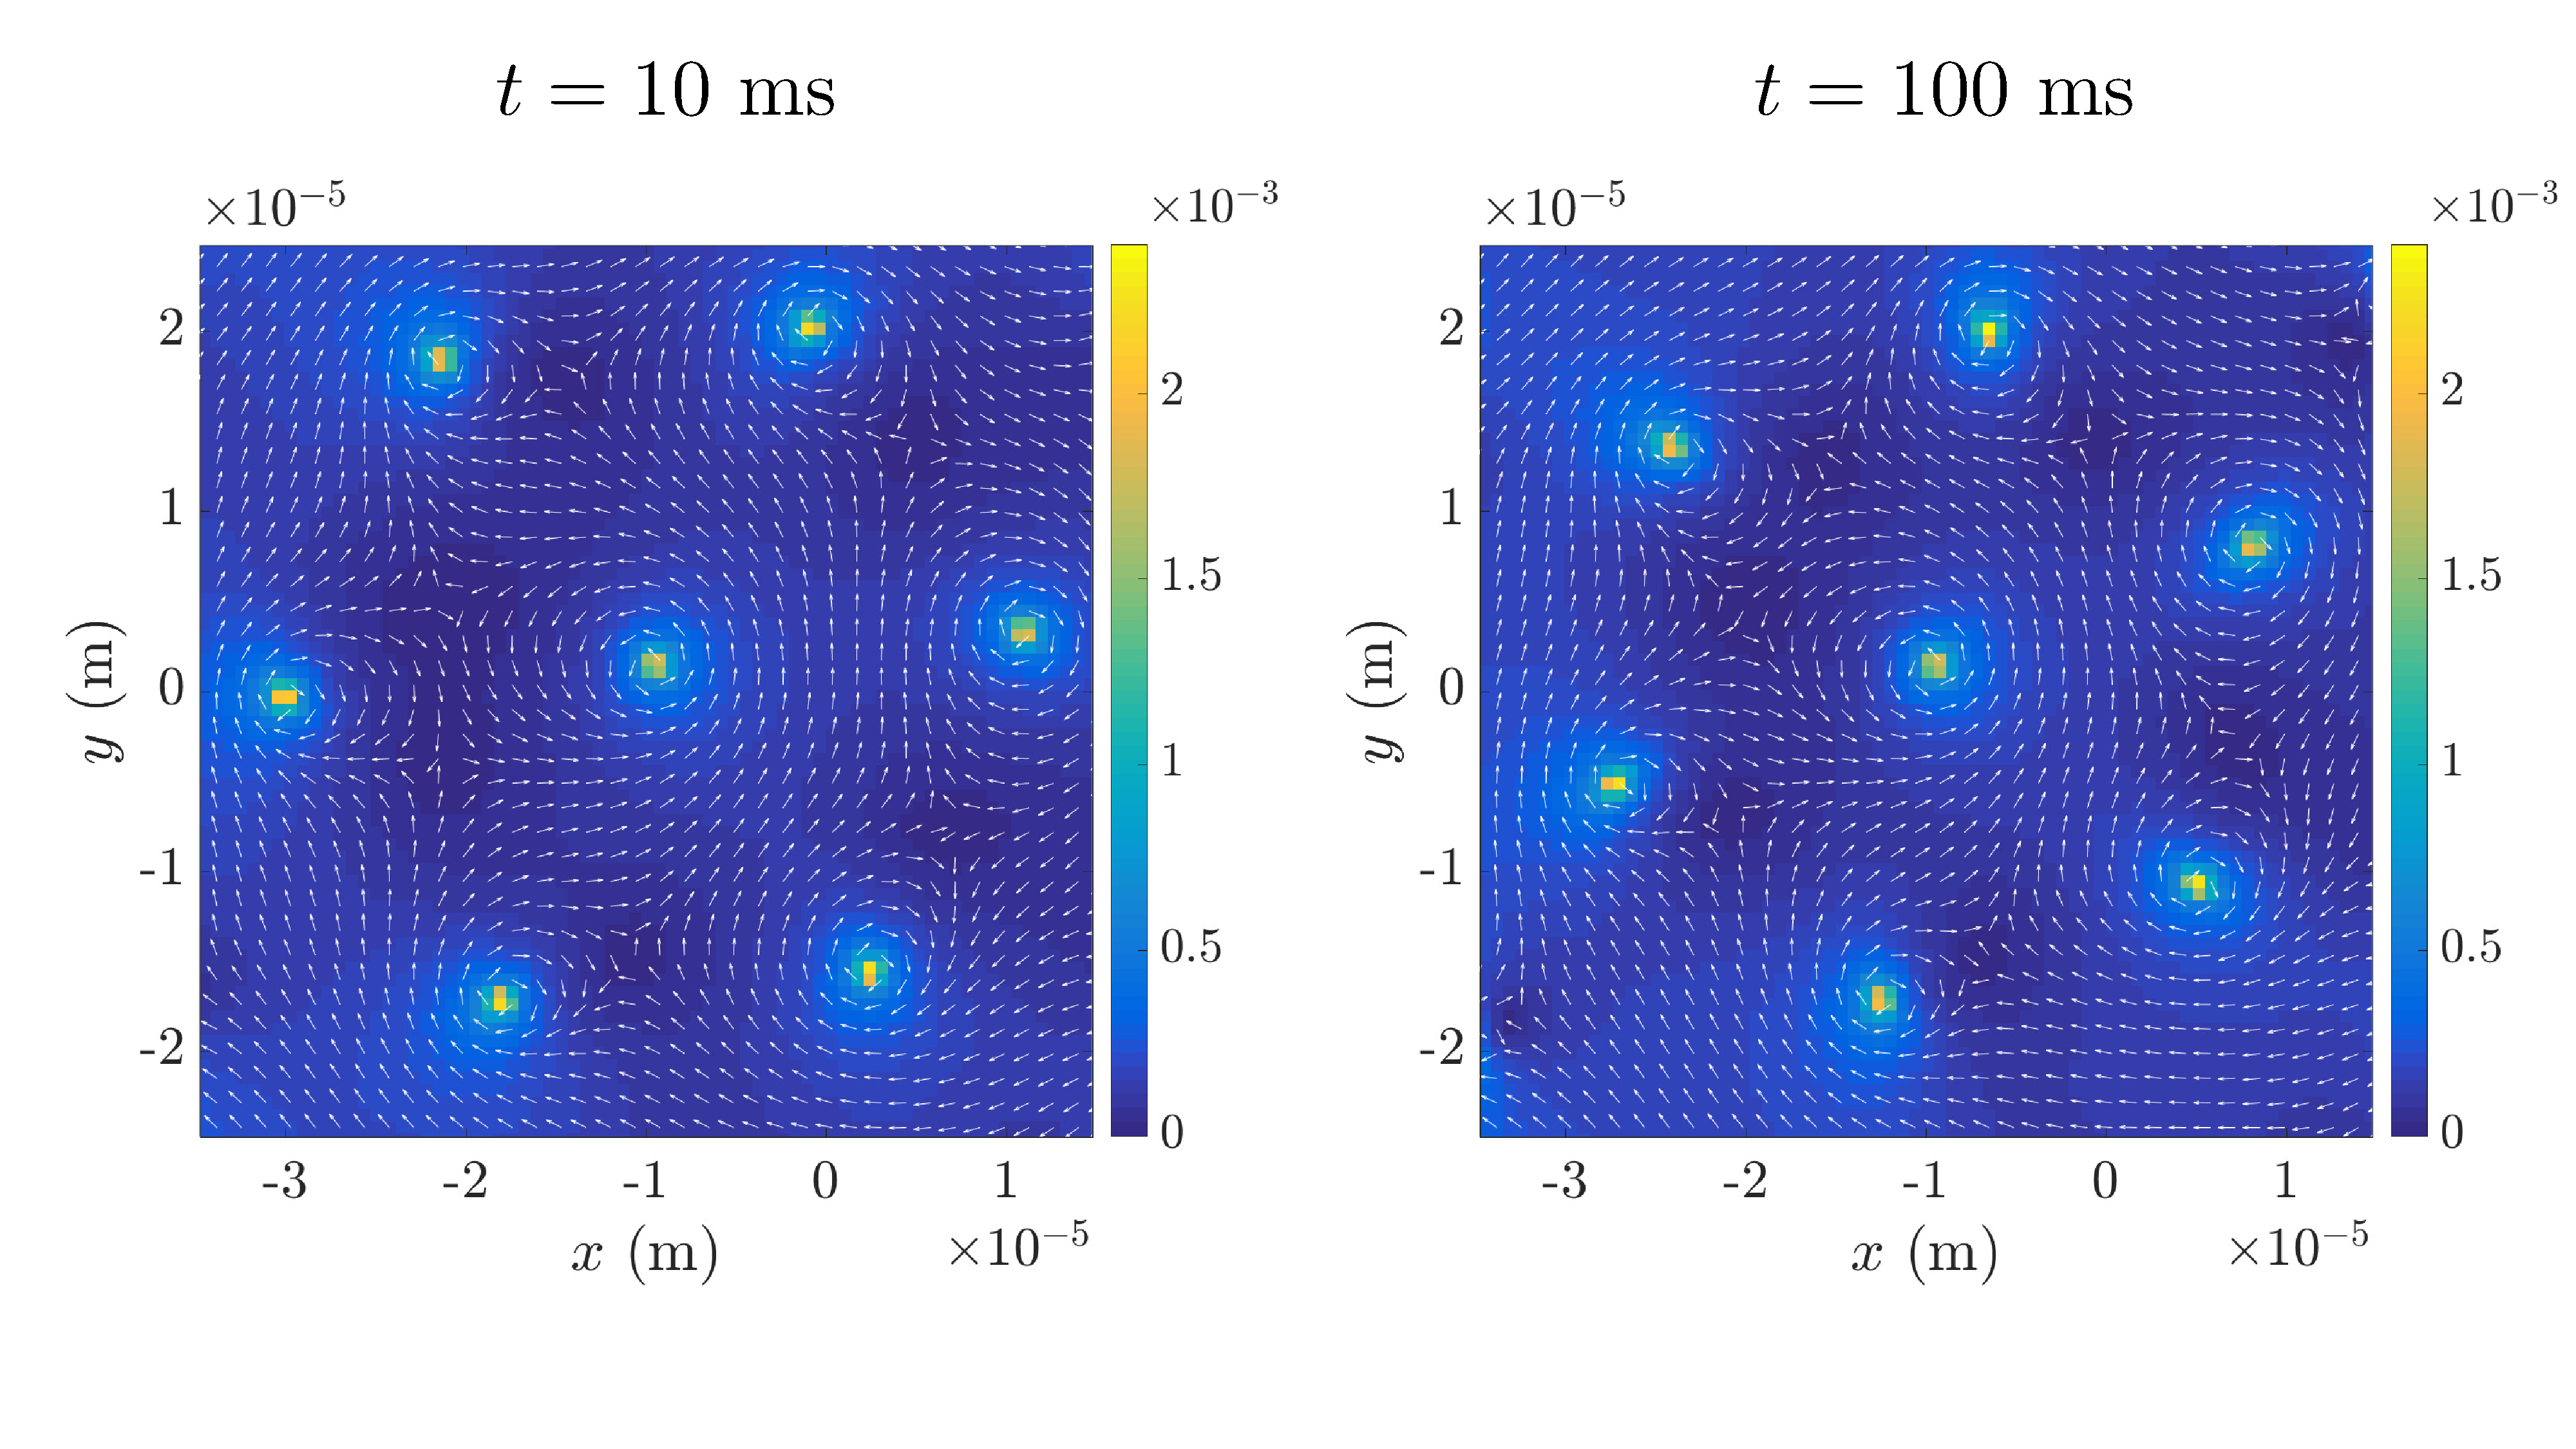
\includegraphics[width=0.95\textwidth]{ch6_phasegineer/velfield/var161anti_velfield}
    \caption{Velocity field of the vortex lattice following the flipping of a vortex to an antivortex for $t=(10,100)$ ms. The change in the velocity field adjacent to the vortex causes the surrounding vortices to rotate at a much slower rate than the solid-body rotation of the vortex lattice. This in turn creates a large change in the resulting ordering of the lattice. The unbalanced local field will eventually lead to the antivortex moving and annihilating with a nearby vortex.}
    \label{fig:varr161anti_velfield}
\end{figure}


\begin{figure}\centering
    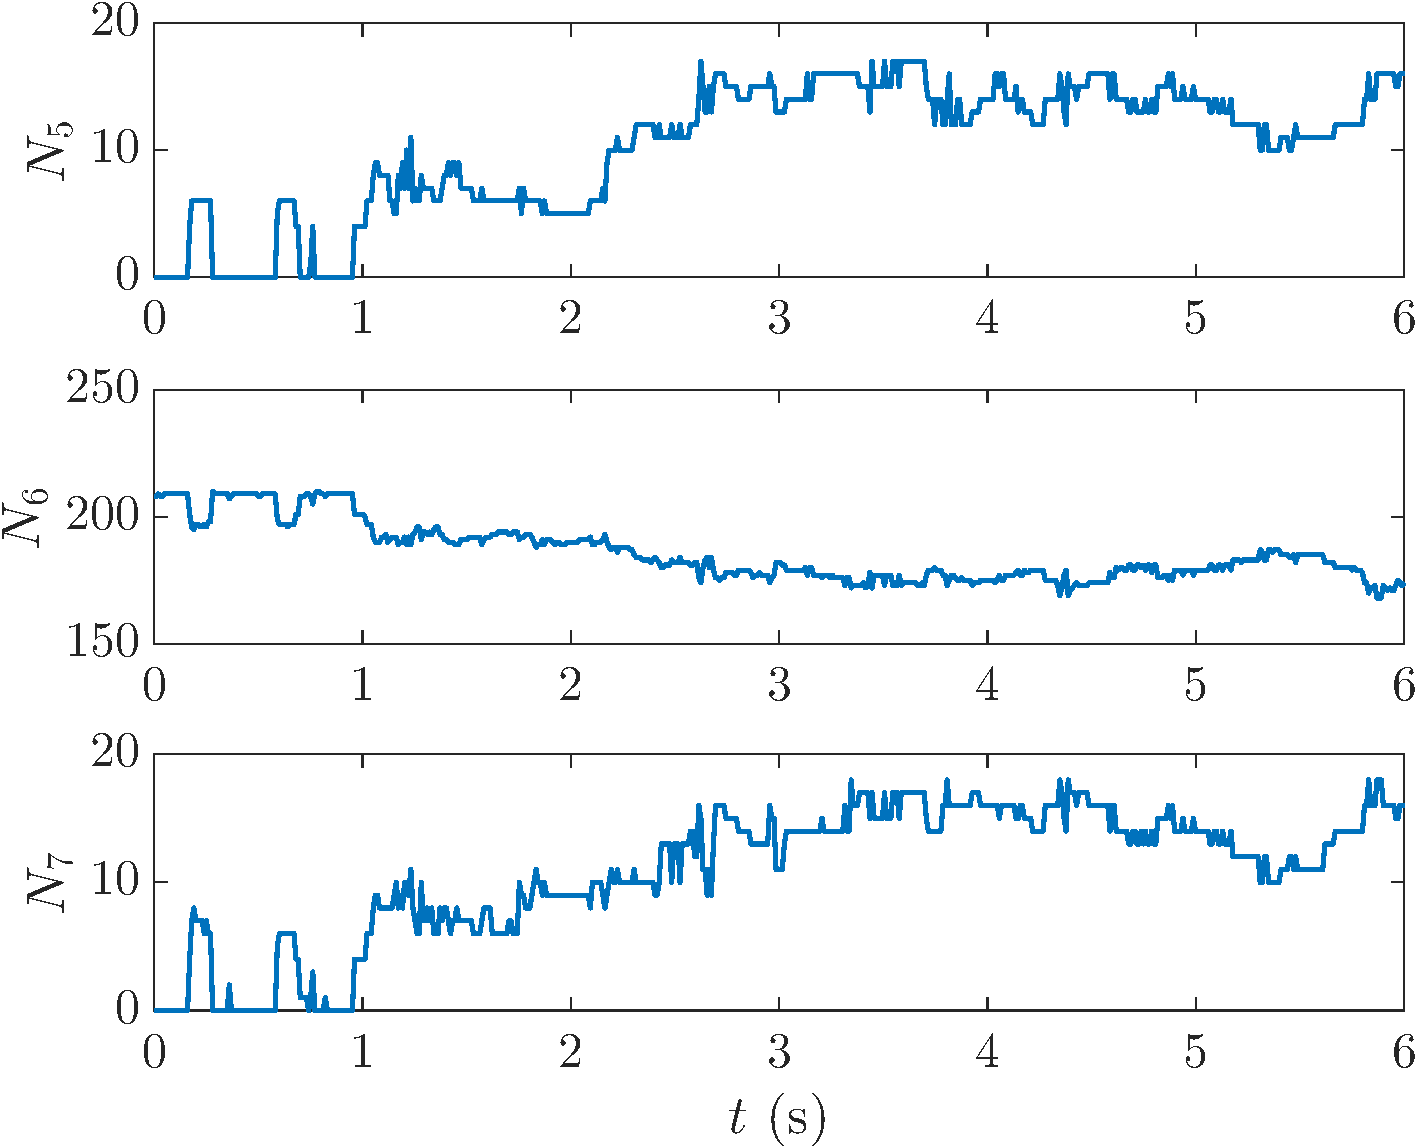
\includegraphics[width=0.5\textwidth]{ch6_phasegineer/arxiv/fig10.pdf}
    \caption{The defect ($N_5,~N_7$) and triangular lattice ($N_6$) nearest neighbour count taken from a Delaunay triangulation of the vortex lattice following the insertion of an antivortex. The number of defects increases as the local structure decays, and eventually gives rise to a quasi-constant state.}\label{fig:varr161anti_defect}
\end{figure}

A final class of possible perturbations is the removal of a cluster of neighbouring vortices from the lattice, and in Fig.~\ref{fig:remove7_defect} we show the results from erasing an entire seven vortex unit cell from the condensate. As expected, one can see that the number of lattice defects rises considerably and does not settle during the time over which we can simulate the condensate. In this case, the disordered regions occupy a large area of the lattice and the number of 6-fold connected vortices becomes very low.

\begin{figure}\centering
    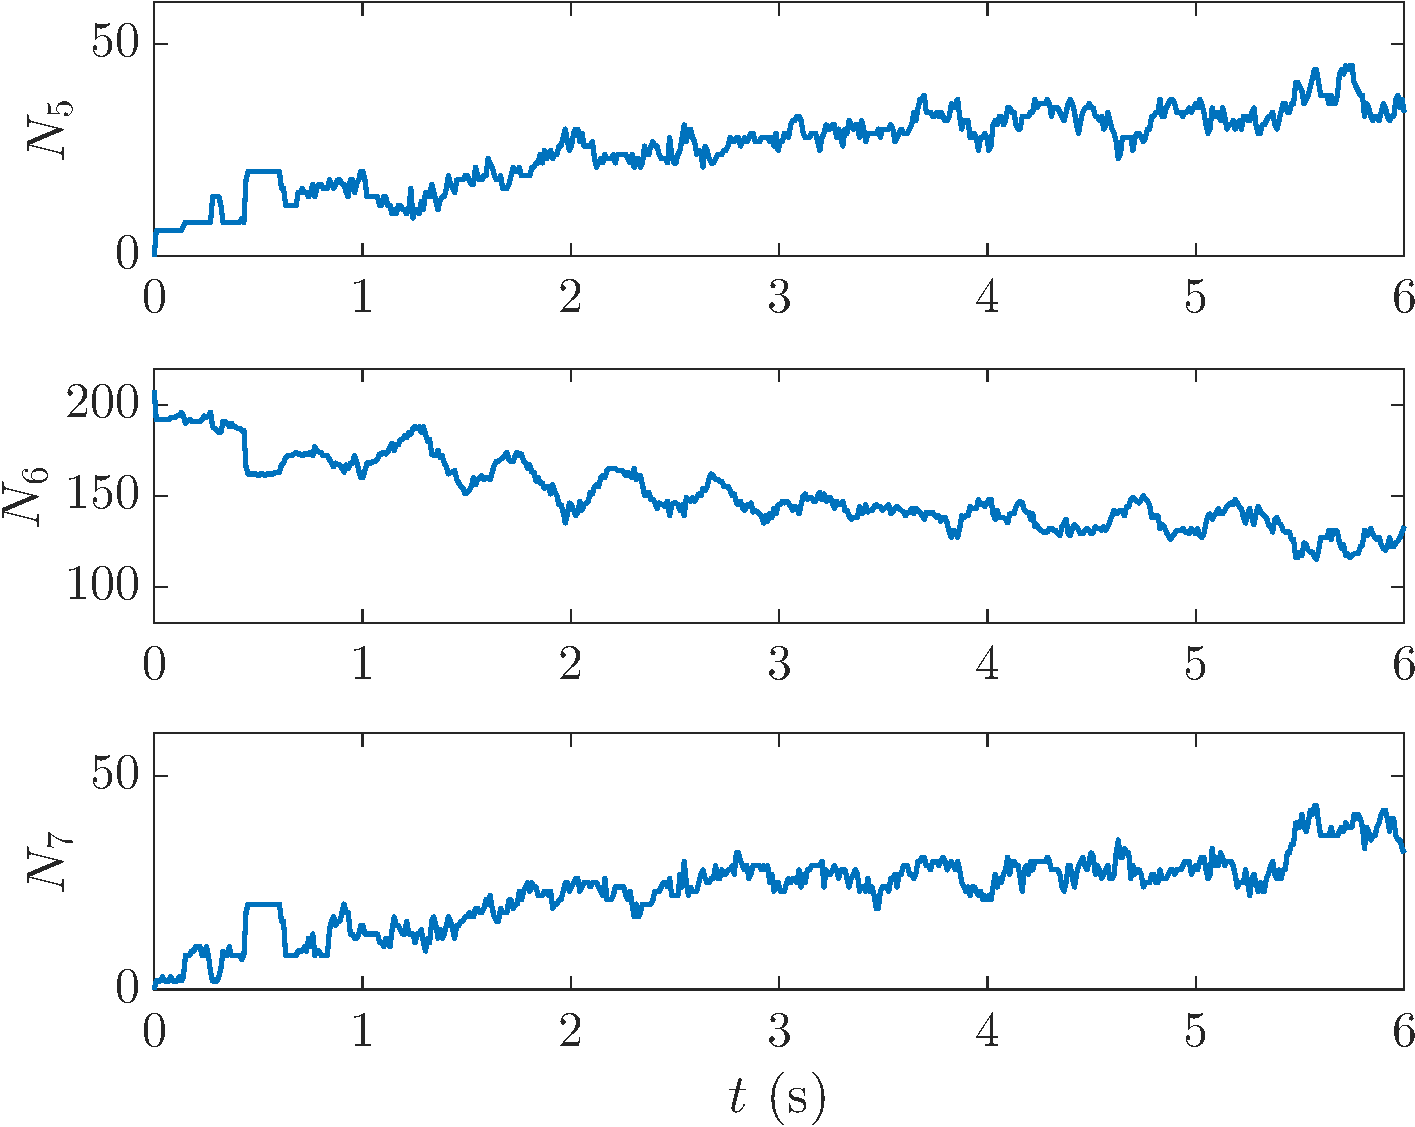
\includegraphics[width=0.5\textwidth]{ch6_phasegineer/arxiv/fig11.pdf}
    \caption{The defect ($N_5,~N_7$) and triangular lattice ($N_6$) nearest neighbour count from a Delaunay triangulation of the vortex lattice following the removal of 7 vortices from the centre of the lattice. }\label{fig:remove7_defect}
\end{figure}

Comparing the orientational correlation function for the three cases discussed in this section (removing two distant vortices, creating an antivortex, and removing 7 vortices) also demonstrates the different degree of disorder they produce (see Fig.~\ref{fig:g6_2edge_anti_nuclear}). The removal of the two vortices at opposite sides of the condensate still yields reasonably high correlations ($\langle g_6(r) \rangle \approx 0.8$) at all times and length scales, indicating a well ordered lattice. Creating an antivortex in the lattice leads to lower correlations across all length scales, especially in the long time limit ($\langle g_6(r) \rangle\approx 0.7$), but still tends to the same long-ranged value as the previous case. This indicates an ordered lattice outside the region of the localized defects. Lastly, the removal of seven vortices shows a significant drop in correlations at all length scales and across both times ($\langle g_6(r) \rangle\approx 0.5$), indicating a global disordering of the vortices, which is consistent with the large number of defects identified earlier.

\begin{figure}\centering
    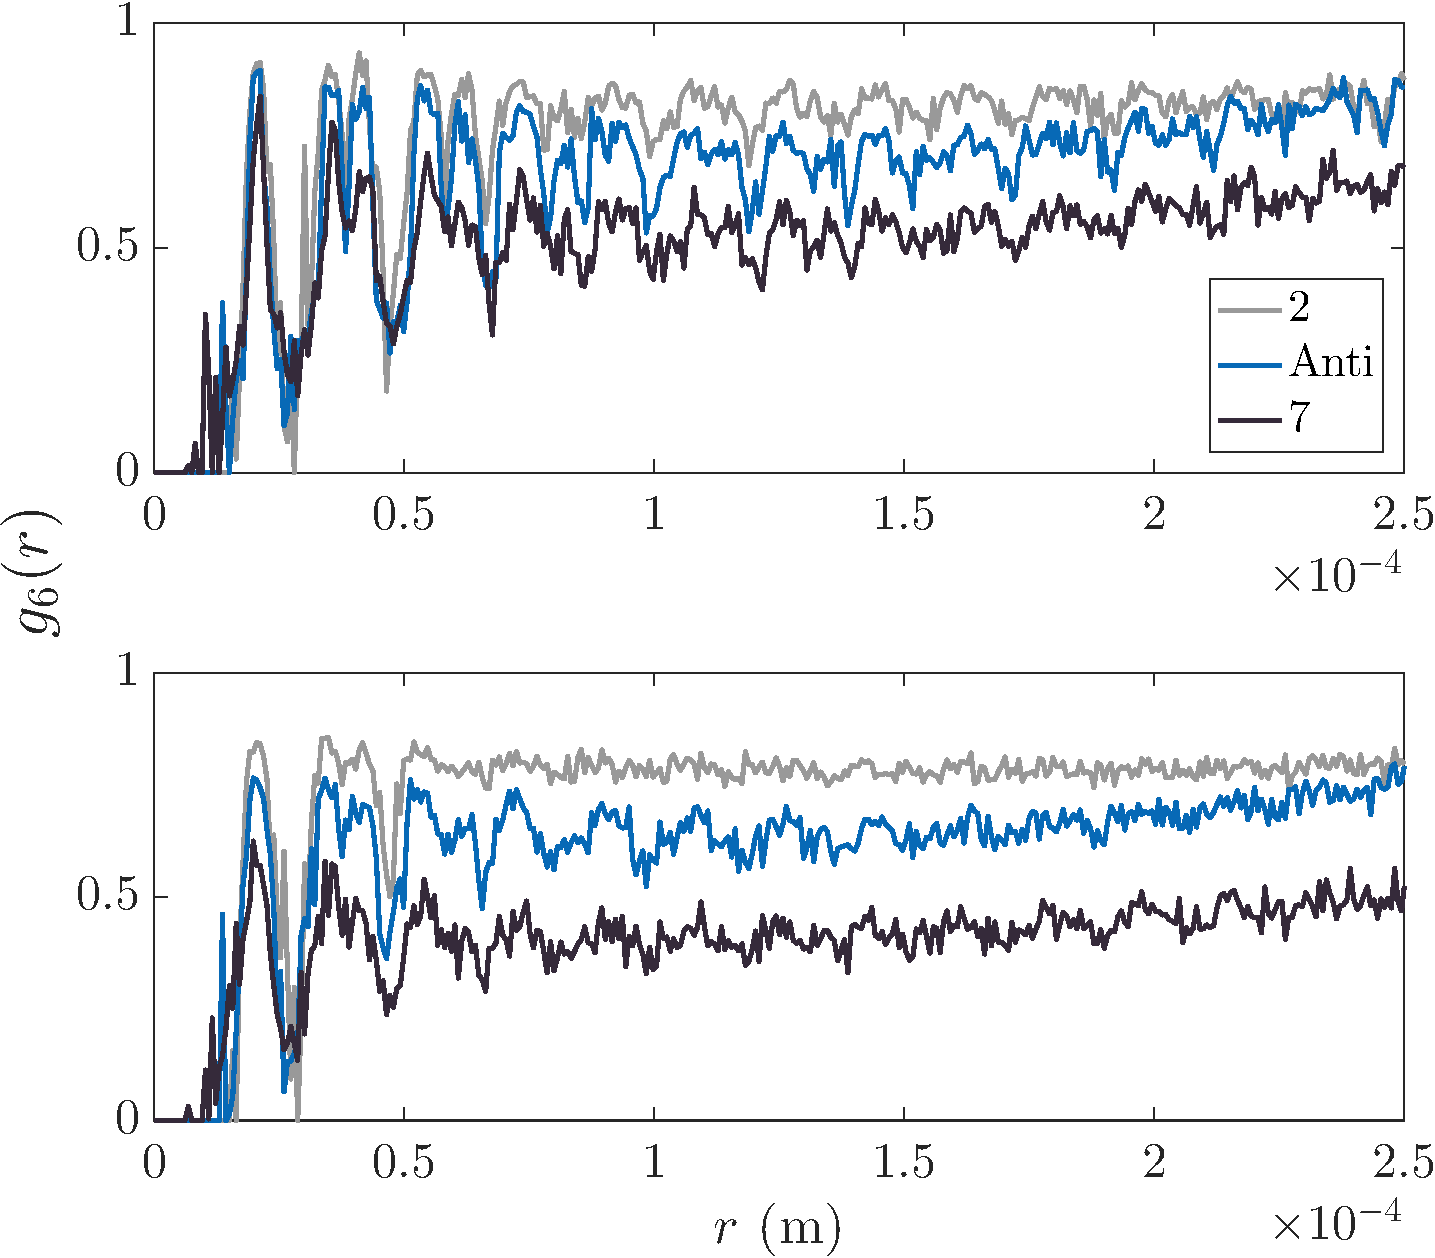
\includegraphics[width=0.5\textwidth]{ch6_phasegineer/arxiv/fig12.pdf}
    \caption{The orientational correlation function is given for moderate ($t=3$ seconds, top) and long ($t=6$ seconds, bottom) times after the phase imprint for removing 2, creating an antivortex, and removing 7 vortices respectively. The general behaviour at short and long ranges is similar for all three scenarios, but the correlations are significantly reduced, especially for the situation where seven vortices are removed.}\label{fig:g6_2edge_anti_nuclear}
\end{figure}

An alternative view of the above dynamics can be given from the Voronoi tessellation of the lattice. For the above cases of $(a)$ removing a vortex from the centre, $(b)$ removing 2 away from the centre, $(c)$ flipping the rotation direction, and $(d)$ removing 7, the ensuing evolutions are shown in Fig.~\ref{fig:voronoisarea}, with the colours representing the vortex cell area. Snapshots are taken at times $t=(0.01,0.1,1,6)$ s, with the mean area $\bar{A}$ and standard deviation $\sigma$ over time also shown. We can use this to observe the perturbation on the lattice, and see how it disturbs positions across the entire condensate. One can see that the perturbation initially affects only the vortices close to the defect. The Voronoi cells within this region have a much larger area than those of the surrounding regions. As the system evolves the defect disturbs the system outward from the initial imprint, with the strength of this disturbance being visible in the change of cell areas. As described earlier, the defect region maintains its honeycomb-like structure for up to $t=1$ s. Rapid oscillations in $\bar{A}$ and a peak in $\sigma$ persist up to approximately $t=1.5$ s, after which they settle into an oscillation at the breathing mode frequency $2\omega_\perp$ and a constant value respectively for cases $(a)$, $(b)$ and $(c)$. The settling of these values is indicative of the lattice vacancy decaying and the lattice settling into a more disordered arrangement. For case $(d)$ the removal affects the entire lattice, with the finer details of settling into a new arrangement now completely overtaken by the large-scale disordering.

\begin{figure}\centering
    \begin{subfigure}{0.6\textwidth}
        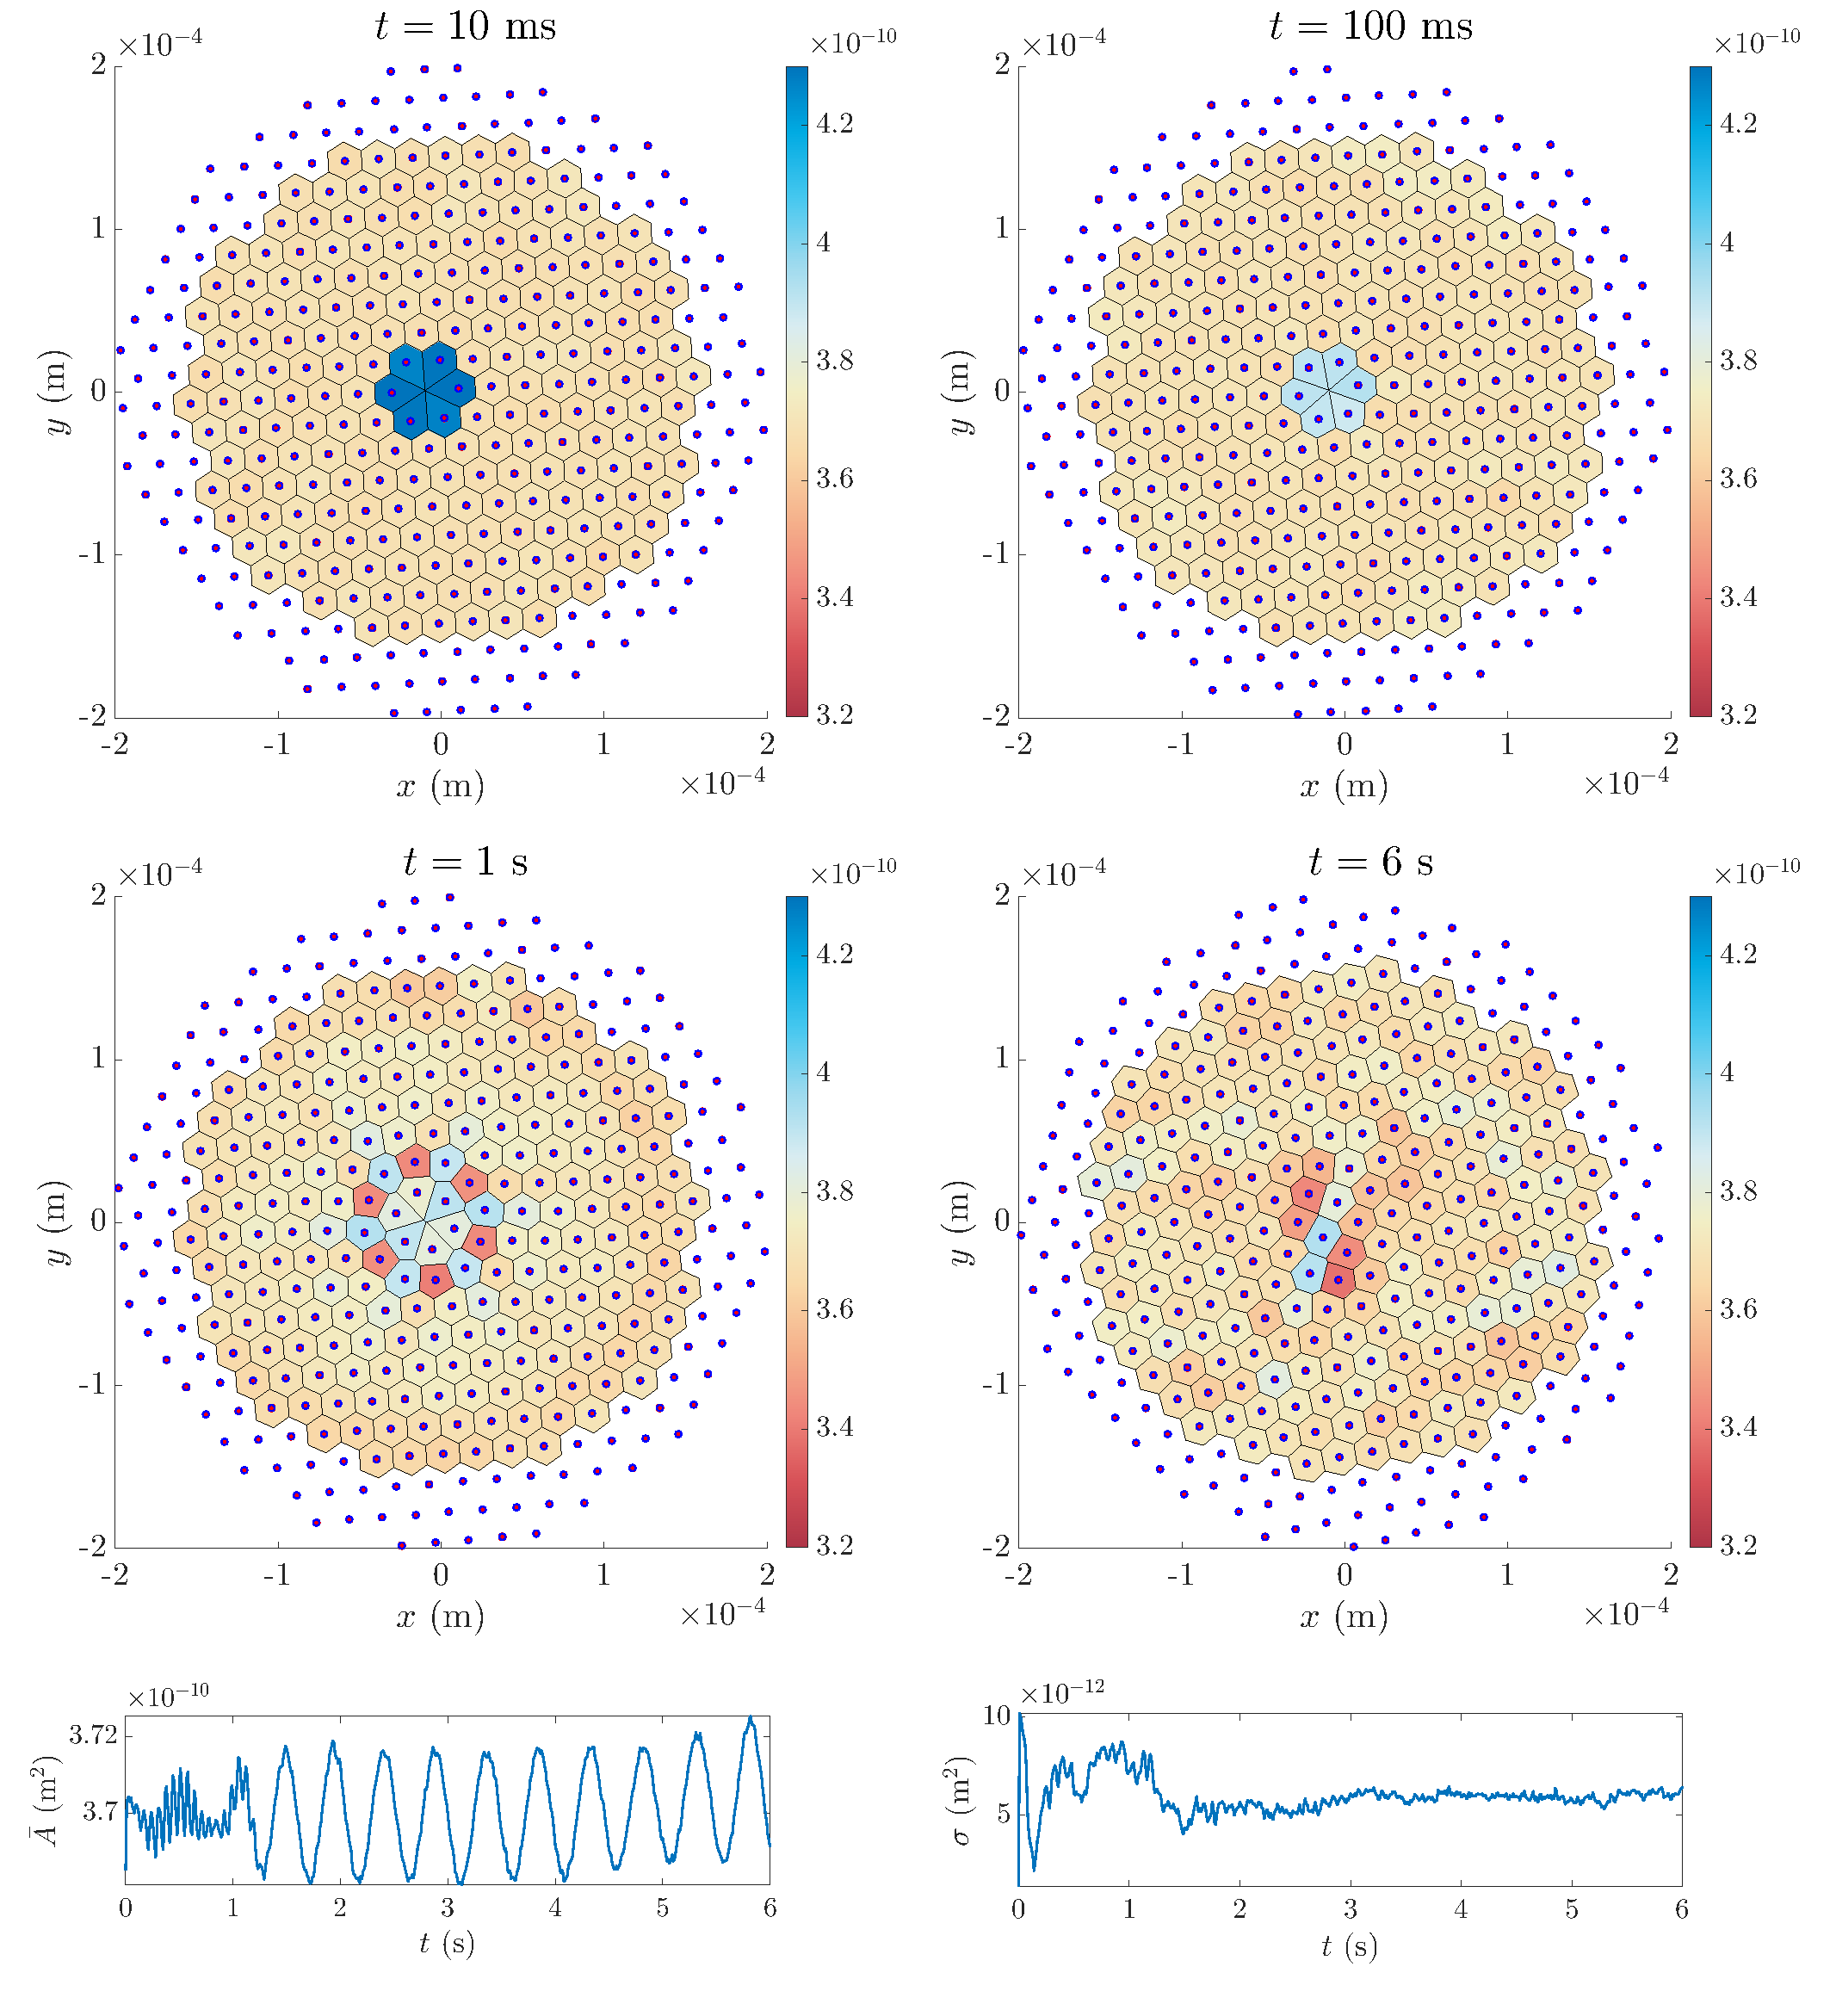
\includegraphics[width=\textwidth,page=1]{ch6_phasegineer/voro/varr_area.pdf}\subcaption{Central vortex removed.}
    \end{subfigure}
    \begin{subfigure}{0.6\textwidth}
        \includegraphics[width=\textwidth,page=2]{ch6_phasegineer/voro/varr_area.pdf}\subcaption{Two vortices away from centre removed.}
    \end{subfigure}
    \caption{Voronoi diagram of a perturbed vortex lattice, with mean cell area $\bar{A}$ and standard deviation $\sigma$ following a phase imprint. The cell colour is indicative of the area spanned by the Voronoi cell.}\label{fig:voronoisarea}
\end{figure}

\begin{figure}\ContinuedFloat\centering
    \begin{subfigure}{0.6\textwidth}
        \includegraphics[width=\textwidth,page=3]{ch6_phasegineer/voro/varr_area.pdf}\subcaption{Central vortex rotation direction flipped.}
    \end{subfigure}
    \begin{subfigure}{0.6\textwidth}
        \includegraphics[width=\textwidth,page=4]{ch6_phasegineer/voro/varr_area.pdf}\subcaption{Central 7 vortex cell removed.}
    \end{subfigure}
    \caption{Voronoi diagram of a perturbed vortex lattice, with mean cell area $\bar{A}$ and standard deviation $\sigma$ following a phase imprint. The cell colour is indicative of the area spanned by the Voronoi cell.}
\end{figure}

We can use the local orientational order parameter $g_6(0) = |\zeta_6(\mathbf{r}_0)|^2$ as the colour scale for the above examples. This is shown in Fig.~\ref{fig:voronoiscorr}, again with the mean-value and standard deviations over time given. As with the Delaunay triangulation, and the orientational correlations one can see that the effects of the perturbations are confined to the region close to the affected vortex site. The loss of triangular symmetry is observed for the cells surrounding the affected sites for $(a)$ and $(b)$, which show an almost identical profile for mean-value and standard deviation. For well separated sites the resulting effects on the lattice can be considered as being independent of one another, due to the local nature of the perturbation. For cases $(c)$ and $(d)$, the local disordering of the regions is much higher, with significant deviation from triangular lattice symmetry for $t=1$ s and beyond. These above methods allow us to clearly identify the effects of the perturbations to the lattice, and are a way towards an understanding of the resulting non-equilibrium dynamics.

\begin{figure}\centering
    \begin{subfigure}{0.6\textwidth}
        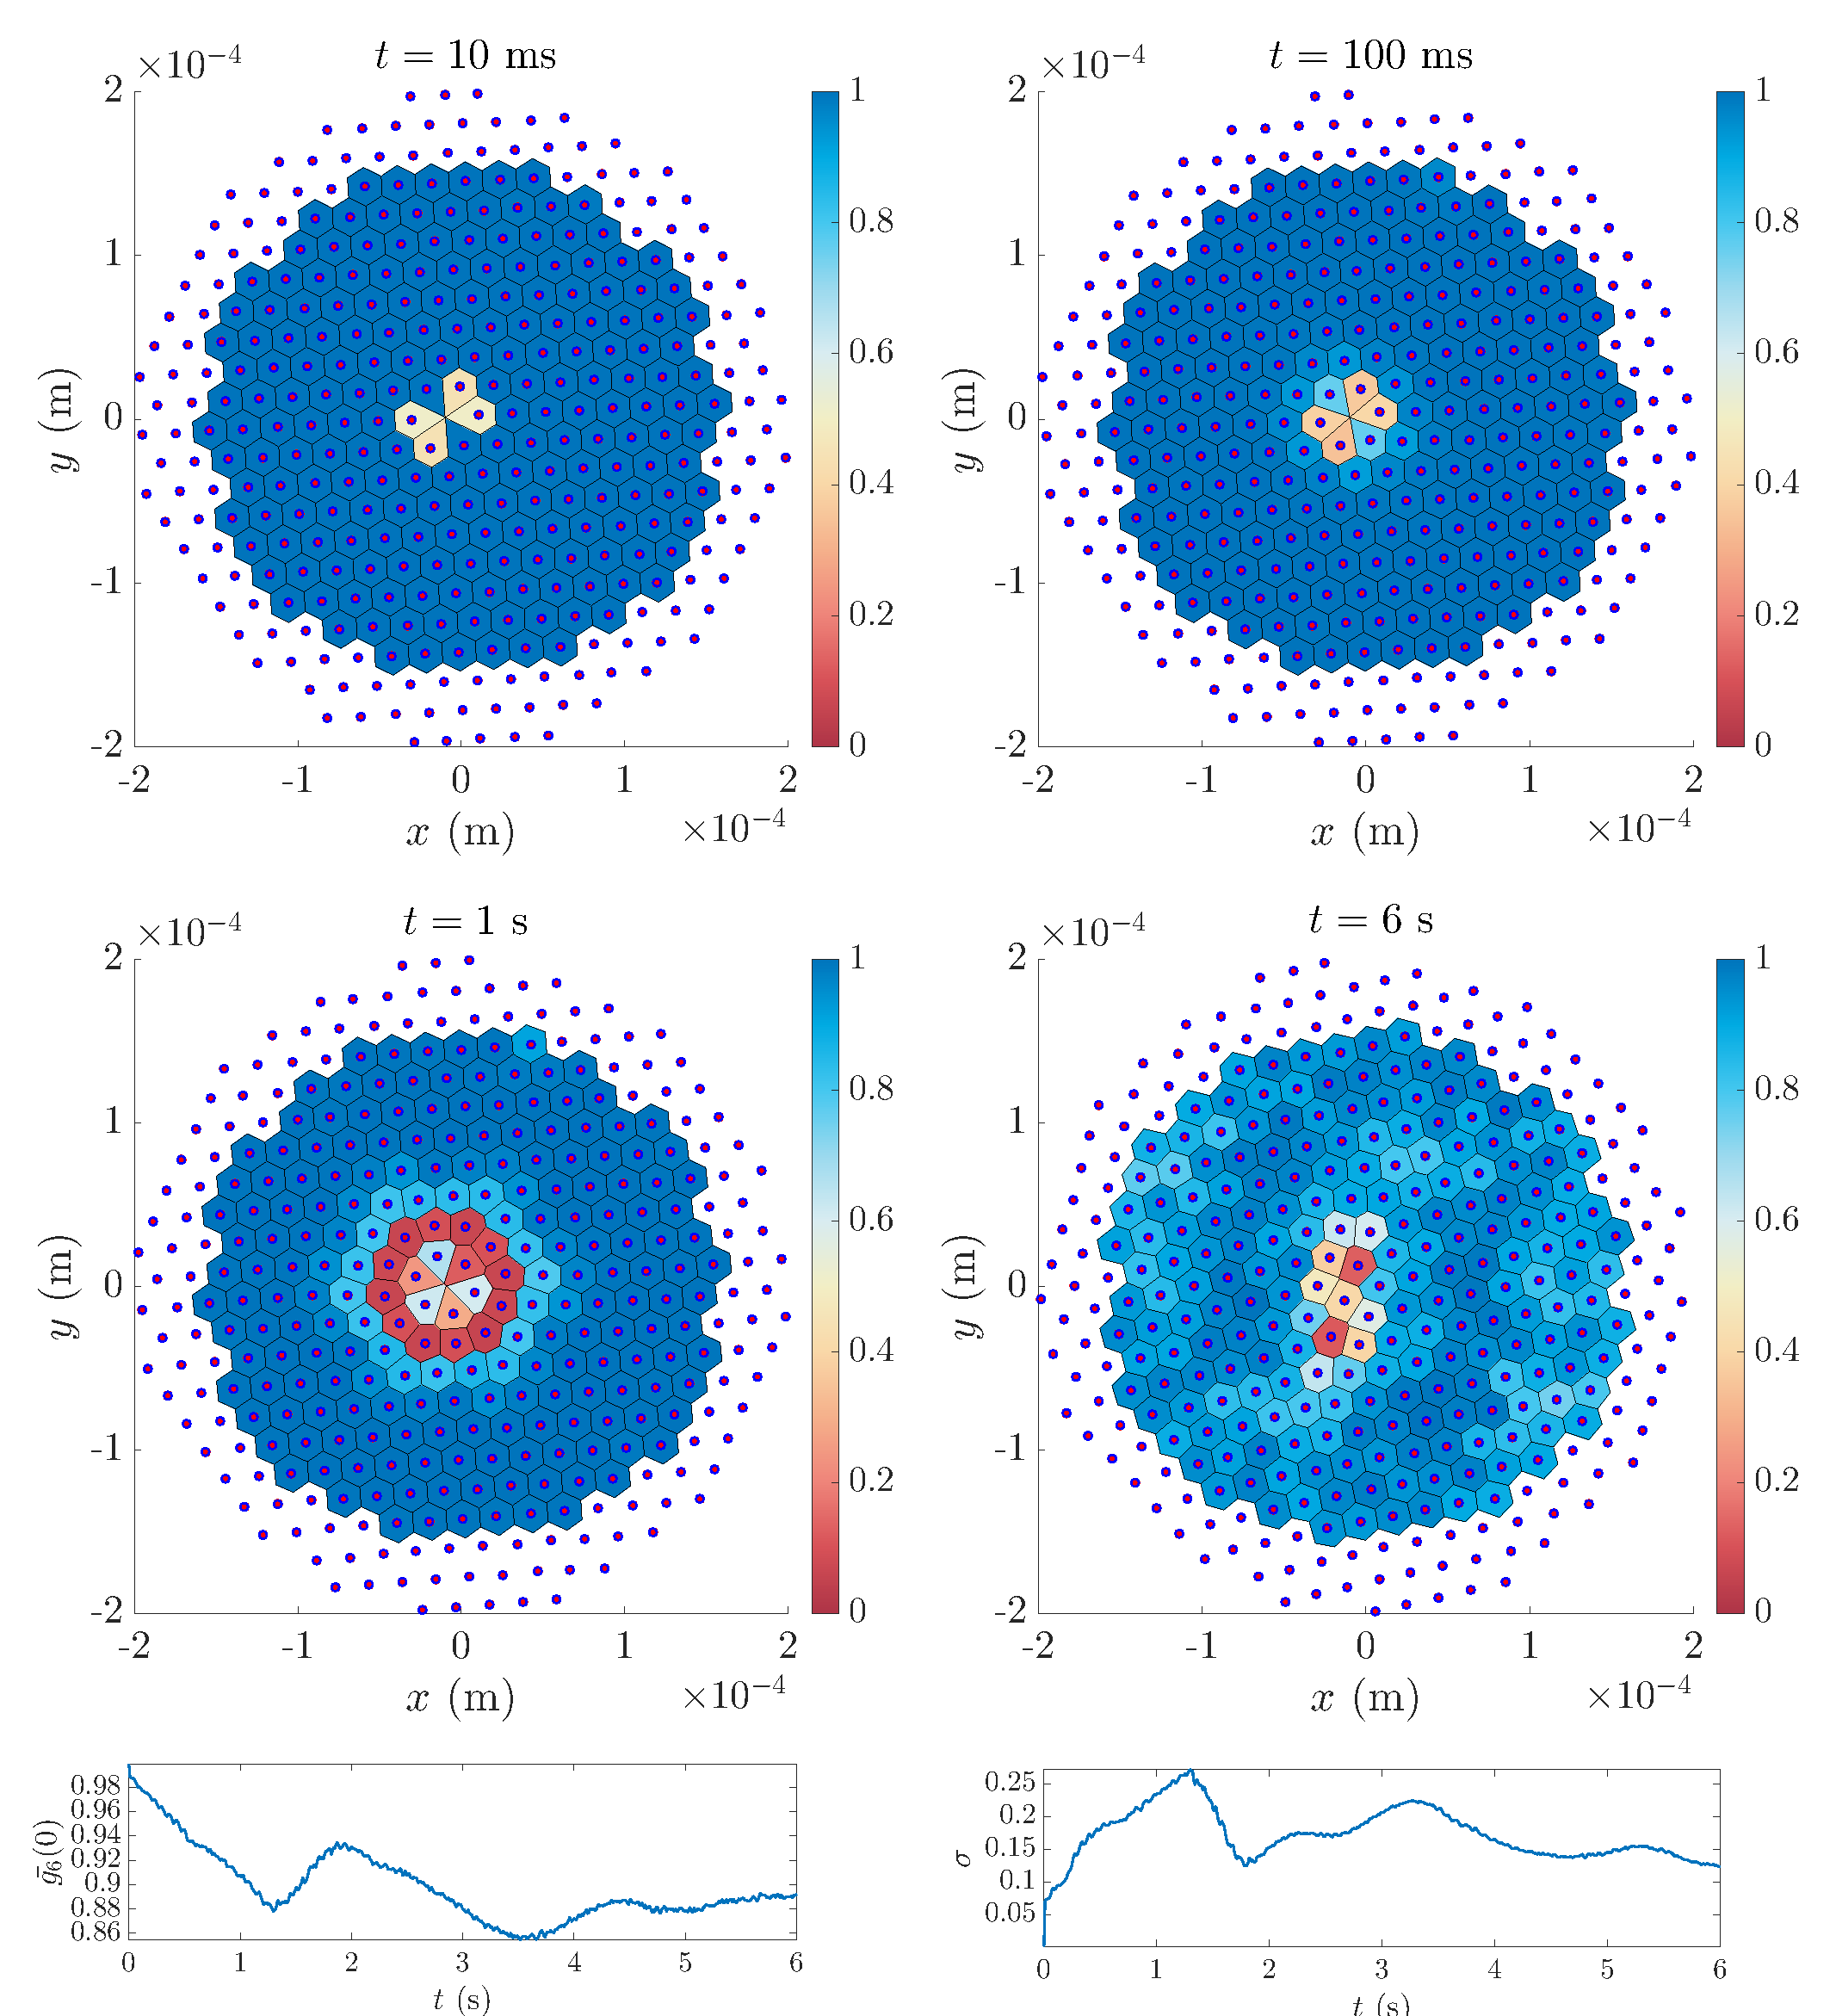
\includegraphics[width=\textwidth,page=1]{ch6_phasegineer/voro/varr_corr.pdf}\subcaption{Central vortex removed.}
    \end{subfigure}
    \begin{subfigure}{0.6\textwidth}
        \includegraphics[width=\textwidth,page=2]{ch6_phasegineer/voro/varr_corr.pdf}\subcaption{Two vortices away from centre removed.}
    \end{subfigure}
    \caption{Voronoi diagram of a perturbed vortex lattice following a phase imprint. The cell colour is indicative of local orientational ordering of the vortex lattice $g_6(0) = |\zeta_6(\mathbf{r}_0)|^2$. The mean value of the local orientational order $\bar{g_6}(0)$ and standard deviation $\sigma$ over time area also given.}\label{fig:voronoiscorr}
\end{figure}

\begin{figure}\ContinuedFloat\centering
    \begin{subfigure}{0.6\textwidth}
        \includegraphics[width=\textwidth,page=3]{ch6_phasegineer/voro/varr_corr.pdf}\subcaption{Central vortex rotation direction flipped.}
    \end{subfigure}
    \begin{subfigure}{0.6\textwidth}
        \includegraphics[width=\textwidth,page=4]{ch6_phasegineer/voro/varr_corr.pdf}\subcaption{Central 7 vortex cell removed.}
    \end{subfigure}
    \caption{Voronoi diagram of a perturbed vortex lattice following a phase imprint. The cell colour is indicative of local orientational ordering of the vortex lattice $g_6(0) = |\zeta_6(\mathbf{r}_0)|^2$. The mean value of the local orientational order $\bar{g_6}(0)$ and standard deviation $\sigma$ over time area also given.}
\end{figure}

\section{Discussion and conclusions}\label{sec:ch6_conc}

We have discussed the situation where controllable amounts of disorder can be created in a BEC vortex lattice through vortex removal or rotational direction flipping at predetermined positions. A single vortex removed from an Abrikosov vortex lattice via phase imprinting creates a quasi-stable honeycomb-like vacancy site. The removal of the associated velocity field near the vacancy, however, disturbs the local solid-body behavior and the vacancy region rotates slower than the surrounding vortex lattice. It eventually decays, creating highly stable topological lattice defects due to the local rearrangement of the vortices, which persist for long times.


In fact, the resulting defects can be seen to pair, with (5,7) lattice defects being the most prominent, and manifesting themselves as dislocation defects in the lattice. Similar behaviour was observed for removing two separated vortices on the lattice, with the resulting defects being independent of one another. This lowered the correlation value, which indicated a drop in the ordering of the vortex lattice. Next, we examined the effect of introducing an anitvortex into the lattice by flipping the phase profile of a pre-existing vortex. The effect of this was to further reduce the order of the vortex lattice, and settle into a lower correlated state than the above cases. Finally, we examined the removal of a large number of adjacent vortices in the lattice, which showed a significant drop in correlations, and hence ordering, over the course of evolution.

The characterization of perturbed lattices put forward by us complements the recent work of Rakonjac \textit{et al.} \cite{VTX:Rankonjac_pra_2016}, where the authors determine the disorder present in a vortex lattice in a BEC by comparing the ratio of the standard deviation of nearest neighbor distances to the mean distance. Here we extend the available tools by using orientational correlations, Delaunay triangulation for topological defect detection, Voronoi tessellation for identifying regions of modified orientational order, and by introducing a method to controllably engineer lattice defects through phase imprinting.

One possible use for the techniques we have discussed is to create vortex turbulence in low-dimensional condensate systems. Contrary to all currently existing discussions, this would make use of the phase erasing technique in Abrikosov lattices to examine turbulence starting from highly ordered systems~\cite{VTX:Neely_prl_2013,VTX:Kwon_pra_2014,VTX:Groszek_pra_2016}. While the use of vortex flipping has been considered previously~\cite{VTX:Madarassy_gfd_2009}, doing this in a highly controllable manner would be advantageous, as one could potentially also investigate phase transitions in the vortex system.

KTHNY (Kosterlitz, Thouless, Halperin, Nelson, Young) theory predicts the melting of two-dimensional systems as a two-step process, where the paired (5,7) defects dissociate, causing a loss of translational correlations, while maintaining quasi-long range orientational order \cite{0022-3719-6-7-010, PhysRevLett.41.121, PhysRevB.19.2457, PhysRevB.19.1855, PhysRevLett.114.035702}. This resulting phase is known as ``hexatic'', and exists between the solid and isotropic liquid phases in two-dimensions. This phase may potentially be observed from the decay profile of correlations in this system. However, given the finite size of this system, observing the hexatic phase may be challenging, as one normally uses the combination of translational correlations as well as orientational correlations to identify this behaviour. In this instance, given the lack of applicability of translational correlations, one might instead opt to examine the structure factor \[S(\mathbf{q}) = \frac{1}{n_v}\displaystyle\sum\limits_{j,k=1}^{n_v} e^{-\textrm{i}\mathbf{q}\cdot(\mathbf{r}_j - \mathbf{r}_k)},\] where $n_v$ is the number of vortices, and $\mathbf{r}_{i,j}$ are the respective vortex positions. The structure factor can be examined for an arc-like profile, which is indicative of the presence of a hexatic phase~\cite{CM:Brodin_cmp_2010,CM:Sun_scirep_2016}. While this was briefly examined (see Fig.~\ref{fig:struct_fact}), conclusive results of such a phase were not initially found. This is likely due to the finite-size of the examined system.

A potential criteria for the onset of the hexatic phase can be given between the stretching and orientational order of nearest neighbouring vortex positions and a Lindemann parameter which quantifies the loss of both translational and orientational order~\cite{CM:Bruun_prb_2014}. Additionally, one can examine the statistics of the endpoints of defect strings, formed between pairs of dislocation (5,7) defects, which can be determined from small particle number systems~\cite{CM:Lechner_prl_2014}. While not examined in the preceding work, these methods can form the basis of a future investigation for the existence of the hexatic phase in the vortex lattice system.

\begin{figure}\centering
    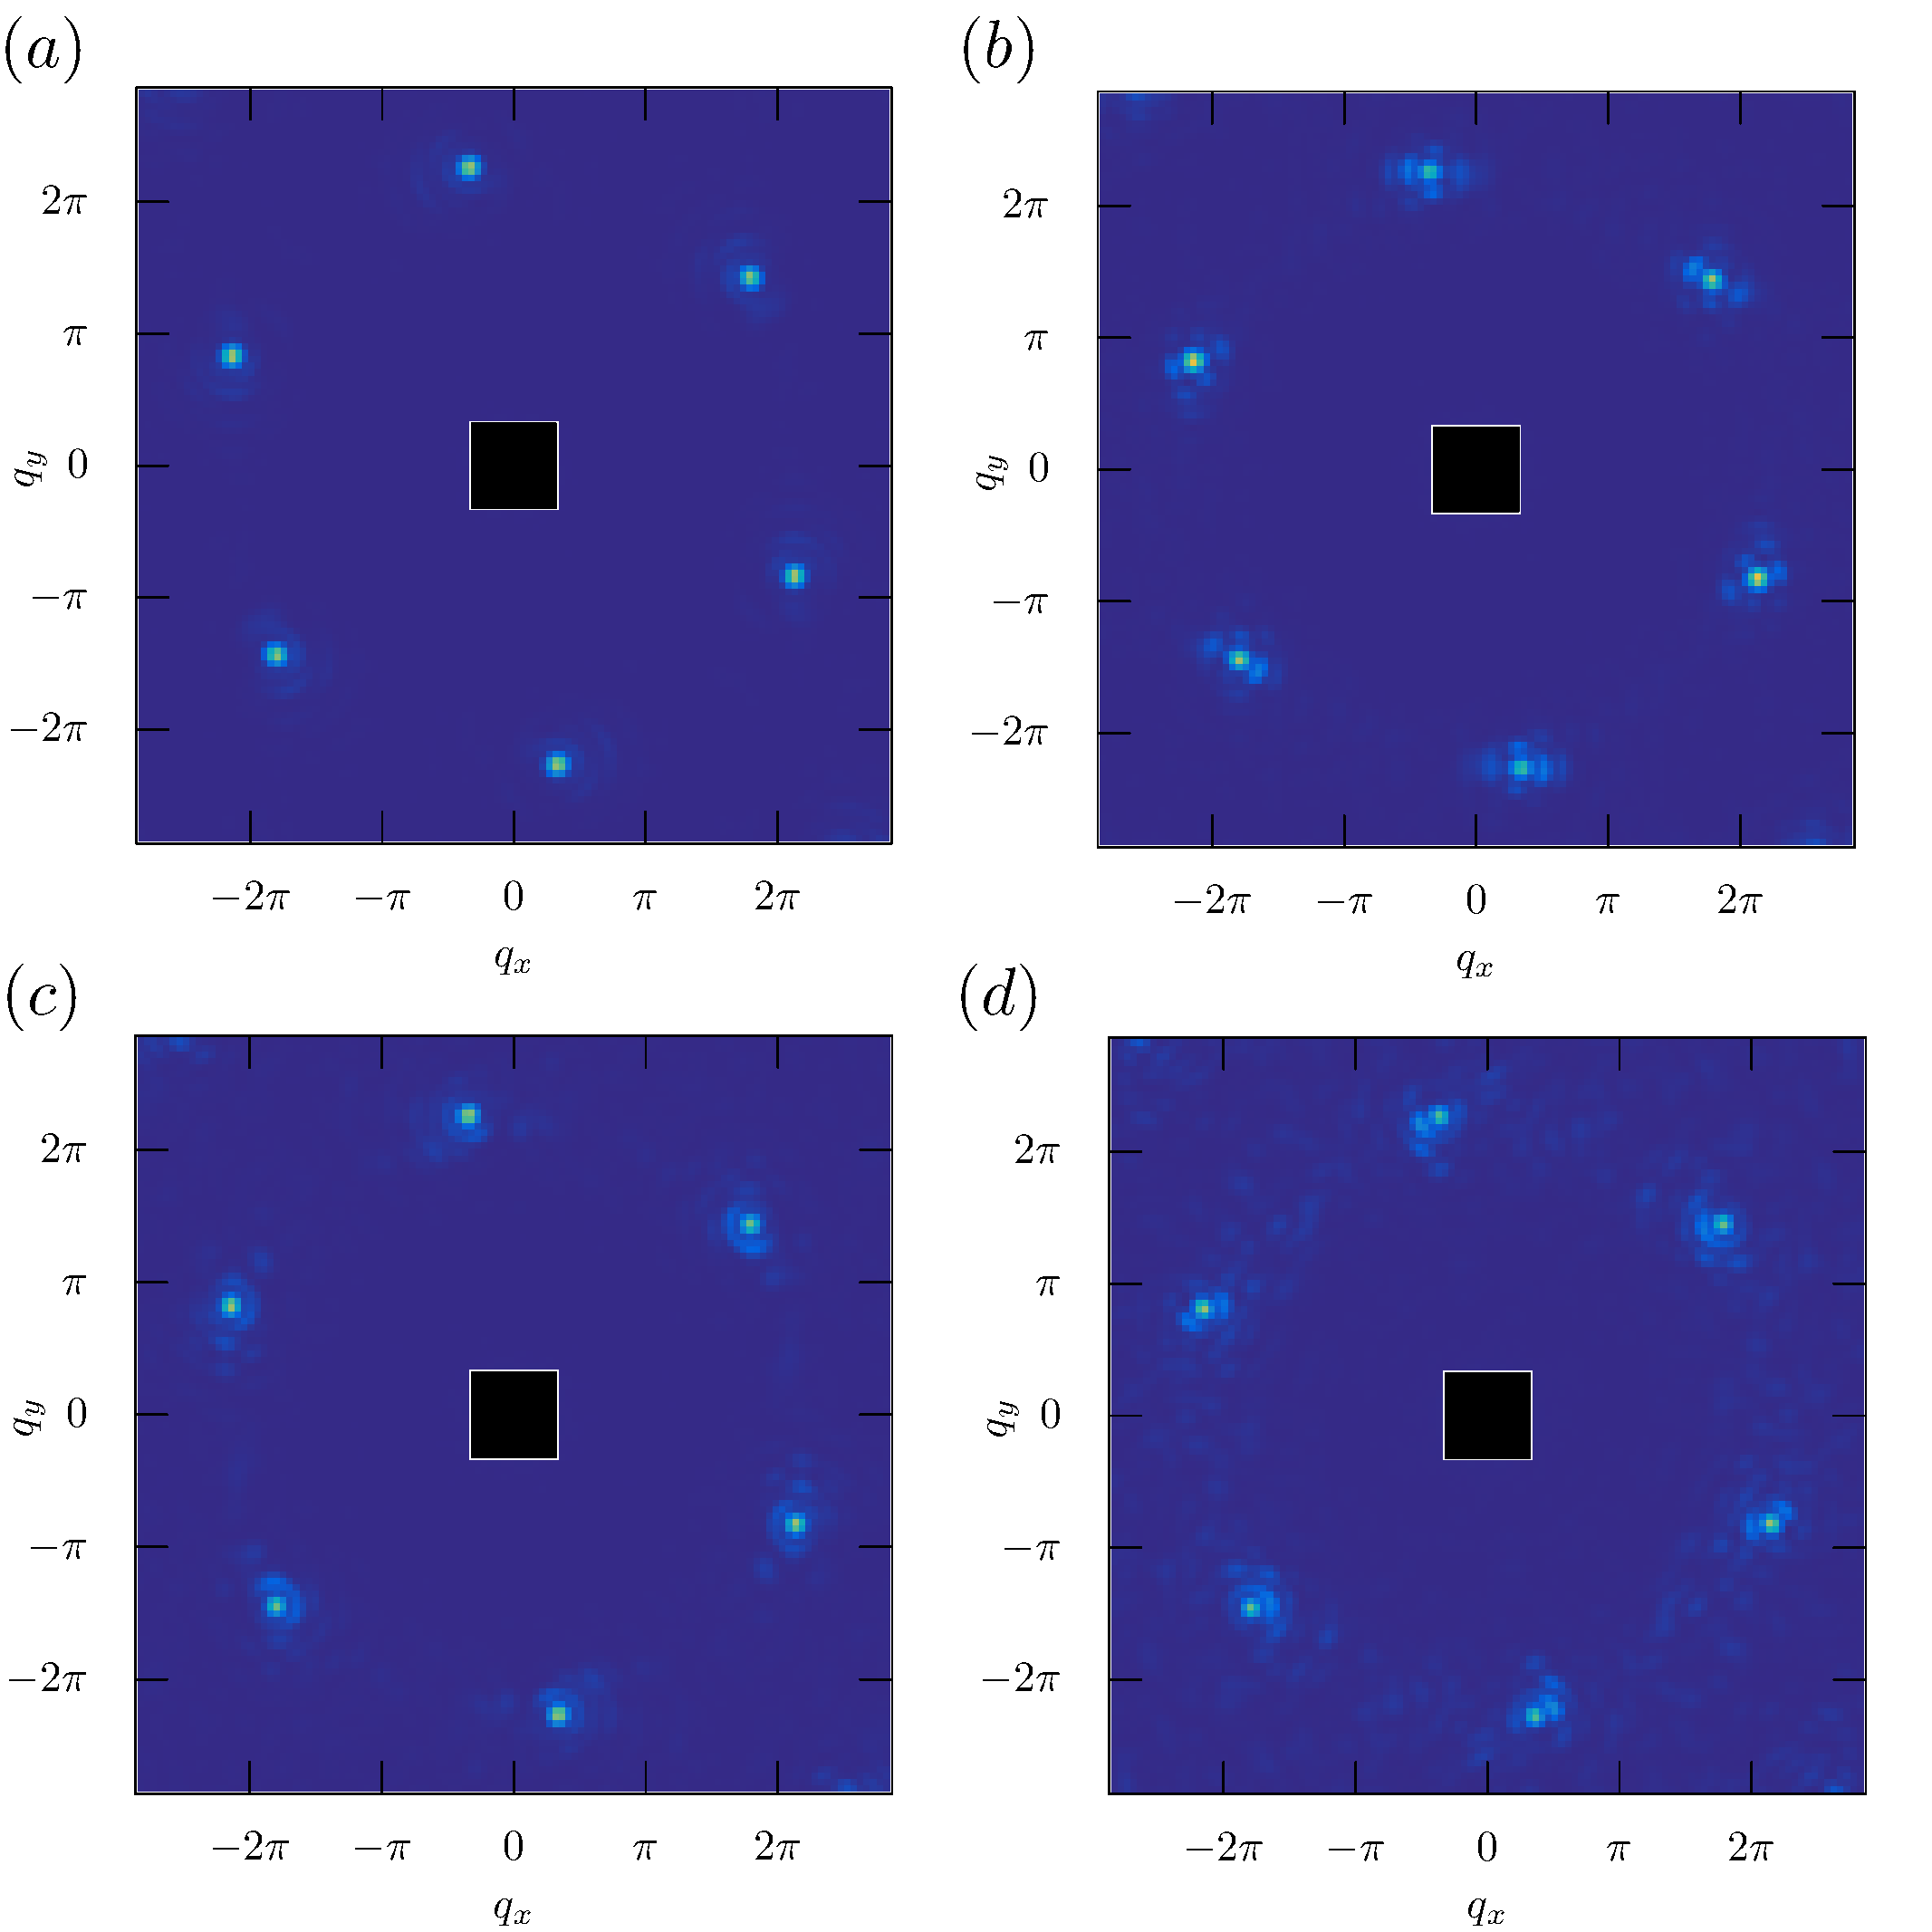
\includegraphics[width=0.5\textwidth]{ch6_phasegineer/structfact.pdf}
    \caption{Structure factor at $t=4$ s for $(a)$ removing central vortex, $(b)$ removing 2 separated vortices, $(c)$ flipping vortex rotation, and $(d)$ removing 7 adjacent vortices. The appearance of a smeared reciprocal peak between that of an amorphous fluid (ring) and a solid (peaks) at the lattice constant can be indicative of a hexatic phase in 2D materials. A continuous smearing of the structure factor peaks cannot be seen, making the determination of a hexatic phase inconclusive. The existence of this phase will require alternative methods to identify the phase, such as those proposed by~\cite{CM:Bruun_prb_2014,CM:Lechner_prl_2014}.}\label{fig:struct_fact}
\end{figure}
